\documentclass{article}
\usepackage{float}
\usepackage{jheppub}
\usepackage{amsmath}
\usepackage{graphicx}
\usepackage{amssymb}
\usepackage{subfig}
\usepackage{natbib}
\bibliographystyle{JHEP-2}
\usepackage[utf8]{inputenc}

\title{Jet-Images -- Deep Learning Edition}
\author{Luke de Oliveira,${}^a$}
\author{Michael Kagan,${}^{b}$}
\author{Lester Mackey,${}^c$}
\author{Benjamin Nachman,${}^{b}$ and}
\author{Ariel Schwartzman${}^b$}

\affiliation{$^{a}$ Institute for Computational and Mathematical Engineering, Stanford University, Stanford, CA 94305, USA}

\affiliation{$^{b}$SLAC National Accelerator Laboratory, Stanford University, 2575 Sand Hill Rd, Menlo Park,
  CA 94025, U.S.A.}

\affiliation{$^{a}$Department of Statistics, Stanford University, Stanford, CA 94305, USA}

\emailAdd{lukedeo@stanford.edu, mkagan@cern.ch, lmackey@stanford.edu, bnachman@cern.ch, sch@slac.stanford.edu}

\abstract{Building on the notion of a particle physics detector as a camera and the jets, or collimated streams of high energy particles, it measures as an image, we investigate the potential of machine learning techniques based on deep learning architectures.  Modern deep learning algorithms trained on {\it jet images} can out-perform standard physically-motivated feature driven approaches to jet tagging.  We develop techniques for visualizing where these features are learned by the network and what additional information is used to improve performance. This feedback loop between physically-motivated feature driven tools and supervised learning algorithms is general and can be used to significantly increase the sensitivity to discover new particles and new forces.}

\begin{document}

\maketitle

\section{Introduction}
Jets, or collimated sprays of particles resulting from the production of high energy quarks, provide a unique handle to search for signs of new physics at the Large Hadron Collider (LHC)~\cite{LHC}.  Specifically, new heavy particles are predicted by a wealth of theories to decay to Standard Model (SM) particles, such as $W^{\pm}$, $Z$, and Higgs bosons, or top quarks, and in doing so impart such SM particles large amounts of energy, or boost.  This boost leads to the collimation of the SM particle's decay products, resulting in the formation of boosted heavy particle jets when the SM particle decays to quarks.   The identification of the underlying particle which produced a boosted jet, or jet tagging, is a fundamental challenge to searching for signs of new physics at the LHC.  Boosted jets have a rich internal substructure which is unlike that of the typical jet backgrounds produced from Quantum Chromo Dynamic (QCD) interactions. There is a wealth of literature addressing the topic of jet tagging by designing physics-inspired features to exploit the jet substructure~\cite{stuff}.  However, in this paper we address the challenge of jet tagging though the use of Machine Learning (ML) and Computer Vision (CV) techniques combined with low-level information, rather than using physics inspired features.  In doing so, we not only improve discrimination power, but also gain new and deep insight into the underlying physical processes that provide discrimination power by extracting information learned by such ML algorithms. 

The analysis presented here is an extension of the jet-images approach, first studied in~\cite{JetImages} and then studied with similar approaches by~\cite{Others}, whereby jets are represented as images with the energy depositions of the particles within the jet serving as the pixel intensities.  When first introduced, jet-image preprocessing techniques, based on the underlying physics symmetries of the jets, were combined with linear Fisher discriminant analysis (FDA) to perform jet tagging and to study the learned discrimination information.  Here, we make use of modern deep neural networks (DNN) architectures, which have been found to outperform competing algorithms in CV tasks similar to jet-tagging with jet-images.  While such DNN's are significantly more complex than FDA, they also provide the capability to learn rich high-level representations of jet-images and to greatly enhance discrimination.  By developing techniques to access this rich information, we can explore and understand what has been learned by the DNN's and subsequently use this to improve our understanding of the physics governing jet substructure.  We also re-examine the jet pre-processing techniques, to specifically analyze the impact of the pre-processing on the physical information contained within the jet.

Since it's first usage by it's current name~\cite{hinton06}, Deep Learning has taken on many forms and seen success in a variety of fields that have traditionally utilized human-engineered features to create classifiers and apply out-of-the-box machine learning algorithms. In particular, the field of Computer Vision has changed drastically. Since the 2012 ILSVRC winning entry by Alex Krizhevsky and the University of Toronto group ~\cite{alexnet}, Deep Learning -- in particular Convolutional Neural Networks -- have taken over vision-based machine learning, consistently showing human and recently super-human levels performance on key baseline datasets. The increasingly widespread availability of GPUs and associated numerical frameworks has made the time intensive estimation procedures associated with deep neural networks more feasible, and allowed the size of models for image tasks to grow exponentially. 
%For example, the Google team's contribution to ILSVRC 2014 -- the GoogLeNet~\cite{googlenet} -- consisted of 22 layers of convolutional black boxes called ``Inception Units'', and set the benchmarks both for accuracy and speed of a model on such a large scale. 

As it relates to our work, we investigate several deep network architectures and focus on  understanding what information and higher level representations a fully connected and a convolutional neural network will learn in the context of High Energy Physics. We let our knowledge of physics guide our investigations into visualization, understanding, and demystification of deep representations for physics. We shed light inside the black-box of deep learning in the context of object identification in boosted jet physics.

This paper is organized as follows:  The details of the simulated data sets and the definition of jet-images are described in Section~\ref{sec:simulation}.    The pre-processing techniques, included new insights into the relationship with underlying physics information, is discussed in Section~\ref{sec:preprocess}.  We then introduce the deep neural network architectures that we us in Section~\ref{sec:arch}.  The discrimination performance and the exploration of the information learned by the DNN's is presented in Section~\ref{sec:studies}.




%With the increased energy of the LHC\cite{LHC}, and the prospects for future higher energy colliders on the horizon, the possibility of finding new high mass particles is of paramount importance.  However, when such TeV scale particles decay to Standard Model (SM) particles, such as top $W^{\pm}$, $Z$, and Higgs bosons,  or top quarks,  they impart large amounts energy, or boost to the SM particles. 

%The fundamental challenge at the energy frontier of particle physics is identifying subtle signals beneath enormous backgrounds. A monumental triumph was the recent discovery of the Higgs boson - a particle that is produced one in every $10^{10}$ collisions at the Large Hadron Collider (LHC). Machine learning techniques have played a key role in all aspects of this search.  At the most basic level, charged particle tracks are reconstructed using pattern recognition techniques, higher level objects, blah blah. 
%
%Techniques built on physically motivated features have succesfully probed the highest energies and smallest scales ever achieved in terestrial experiments.  At the same time, there have been significant gains 
%
%The high particle multiplicity final states of hadron collider events 
%Something like ``we have figured out many cool variables" "machine learning can find variables"  "lets use one to inform/improve the other!''
%
%Places where ML is used in HEP: TMVA~\cite{Hocker:2007ht}
%
%b-tagging: MV1 (ATLAS) and CSV (CMS)
%tau-tagging
%NP searches
%rare SM measurements (e.g. single top)
%Higgs
%
%Jet Images paper: http://arxiv.org/abs/1407.5675
%
%
%Let's keep a running document with all pub-ready plots in here.

\section{Simulation Details}
\label{sec:simulation}

In order to study jet images in a realistic scenario, we use Monte Carlo (MC) simulations of high energy particle collisions. One important jet tagging application is the identification of highly Lorentz boosted $W$ bosons decaying into quarks amidst a large background from the generic production of quarks and gluons.  This classification task has been thoroughly studied experimentally\footnote{There is also an extensive literature on phenomenological studies - see references within the experimental papers.}~\cite{Khachatryan:2014vla,ATL-PHYS-PUB-2015-033,ATL-PHYS-PUB-2014-004} and used in many experimental analyses~\cite{Aad:2015owa,Khachatryan:2014hpa,Khachatryan:2015mta,Khachatryan:2015oba,Khachatryan:2015gza,Khachatryan:2015bma,Khachatryan:2015cwa,Khachatryan:2015ywa,Aad:2014wea,Aad:2015agg,Aad:2015kna,Aad:2015ufa,Aad:2014haa}.  

To simulate highly boosted $W$ bosons, a hypothetical $W'$ boson is generated and forced to decay to a hadronically decaying $W$ boson ($W\rightarrow qq'$) and a $Z$ boson which decays invisibly ($Z\rightarrow \nu\bar{\nu}$).  The mass of the $W'$ boson determines the Lorentz boost of the $W$ boson in the lab frame since the $W'$ is produced nearly at rest and the $W$ boson momentum is approximately $m_{W'}/2$.  Multijet production of quarks and gluons is simulated as a background.  Both the $W'$ signal and the multijet background are generated using \textsc{Pythia} 8.170~\cite{Pythia8,Pythia} at $\sqrt{s}=14$ TeV.  The angular separation of the $W$ boson decay products in the plane transverse to the beam direction scales as $2m_{W}/p_{T,W}$, where $m_W\approx 80$~GeV and $p_{T,W}$ is the component of the $W$ boson momentum in this plane.  The tagging strategy and performance depend strongly on $p_{T,W}$, so we focus on a particular range: $250$~GeV~$<p_{T,W}<300$~GeV.  This corresponds to an angular spread of about $1$ radian.  The decay products of the $W$ bosons as well as the background are clustered into jets using the anti-$k_t$ algorithm~\cite{antiktpaper} via \textsc{FastJet}~\cite{fastjet} 3.0.3.  To mitigate the contribution from the underlying event, jets are are trimmed~\cite{trimming} by re-clustering the constituents into $R=0.3$ $k_t$ subjets and dropping those which have $p_T^\text{subjet}<0.05\times p_T^\text{jet}$. 

To model the discretization and finite acceptance of a real detector, a calorimeter of towers with size $0.1\times 0.1$ in $(y,\phi)$ extends out to $y=5.0$.  The total energy of the simulated particles incident upon a particular cell are added as scalars and the four-vector $p_j$ of any particular tower $j$ is given by

\begin{align}
\label{eq:calo}
p_j = \sum_{i\text{ incident on $j$}}E_i(\cos\phi_j/\cosh y_j,\sin\phi_j/\cosh y_j,\sinh y_j/\cosh y_j,1).
\end{align}


\begin{figure}[bt]
  \begin{center}
      \subfloat[Unweighted $p_T$ distribution \label{subfig:unweighted_pt}]{
        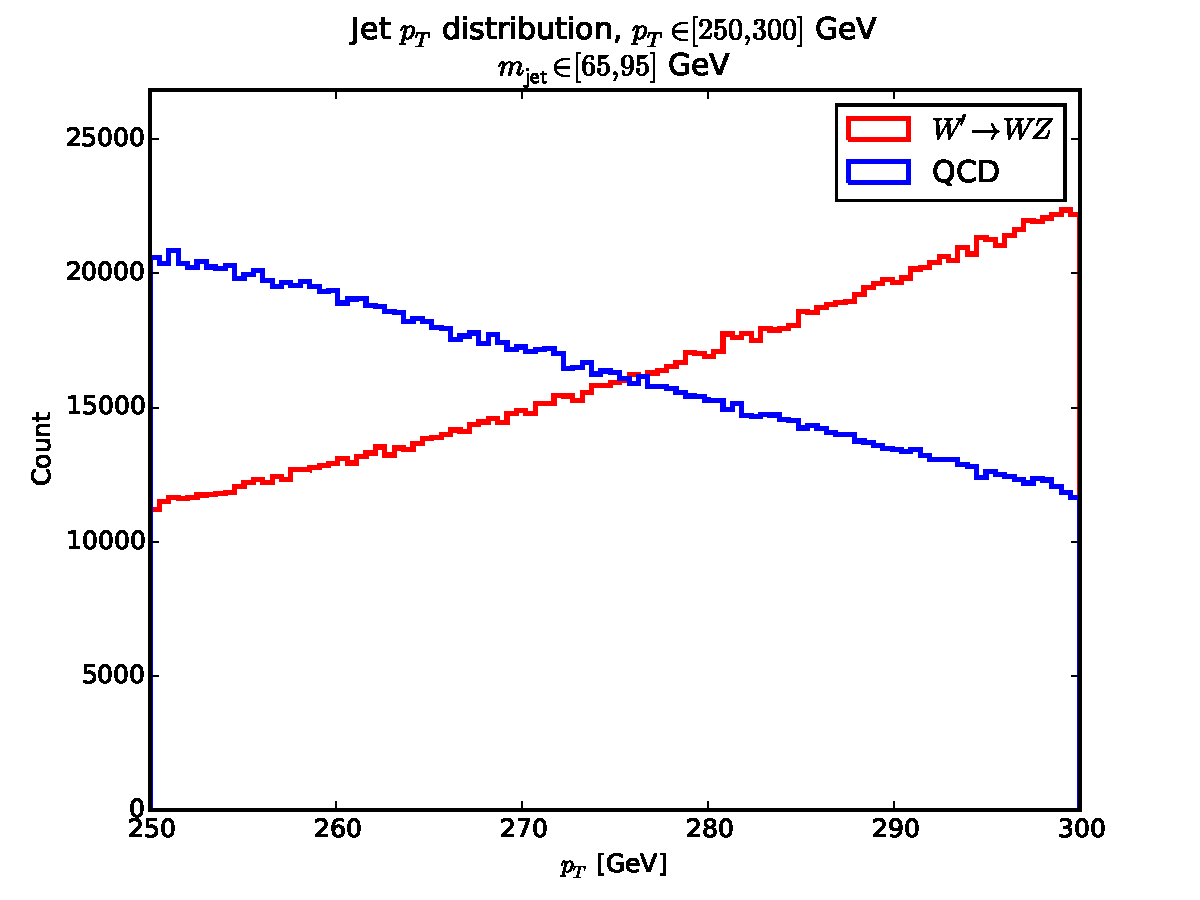
\includegraphics[width=0.5\textwidth]{figures/unweighted-pt-distribution-[250-300].pdf}
      }
      \subfloat[Weighted $p_T$ distribution \label{subfig:weighted_pt}]{
        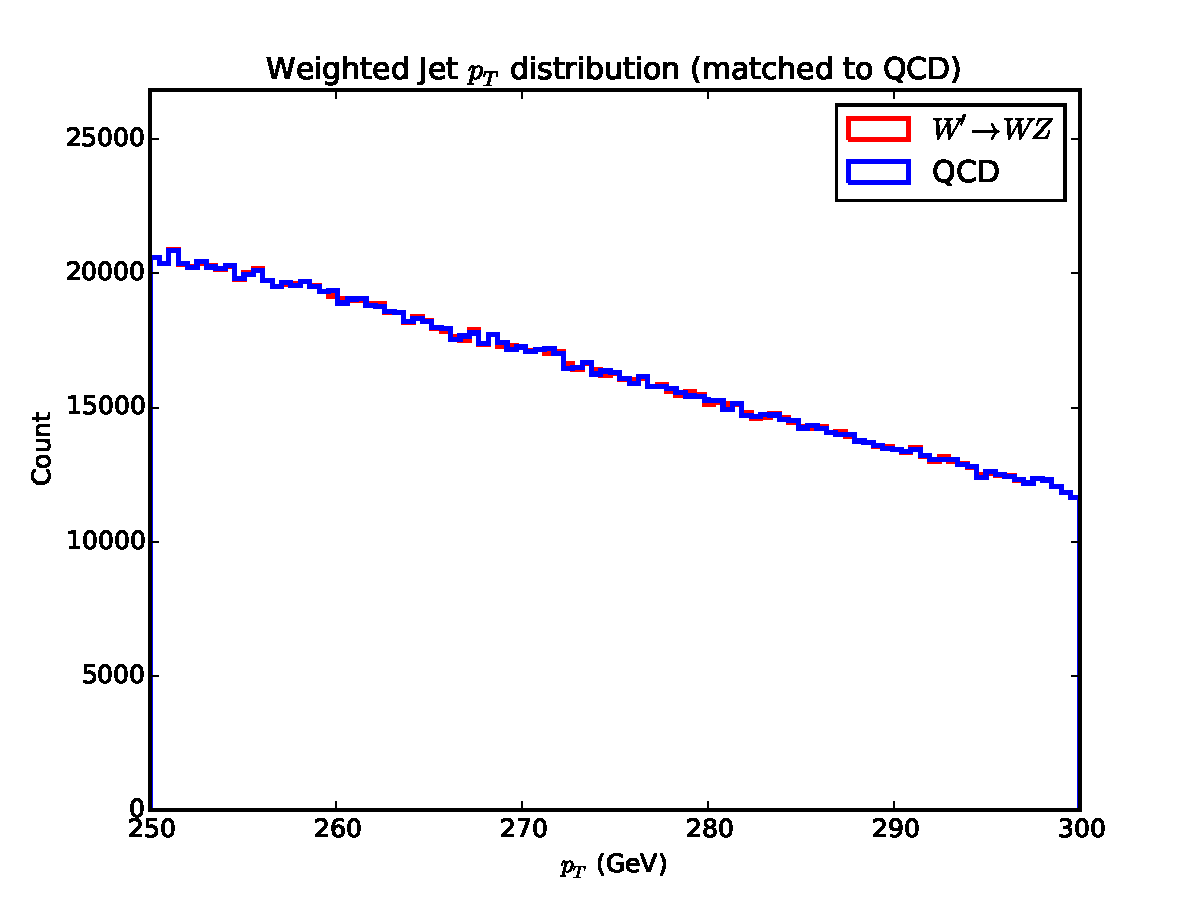
\includegraphics[width=0.5\textwidth]{figures/weighted-pt-distribution[250-300].pdf}
      }
      \caption{ Jets originating from the $W'\rightarrow WZ$ decay are re-weighted such that their $p_T$ spectrum matches that of QCD jets\label{fig:pt} }
    \end{center}
\end{figure}


\begin{figure}[bt]
  \begin{center}
  
  
      \subfloat[Weighted jet mass distribution \label{subfig:weighted_mass}]{
        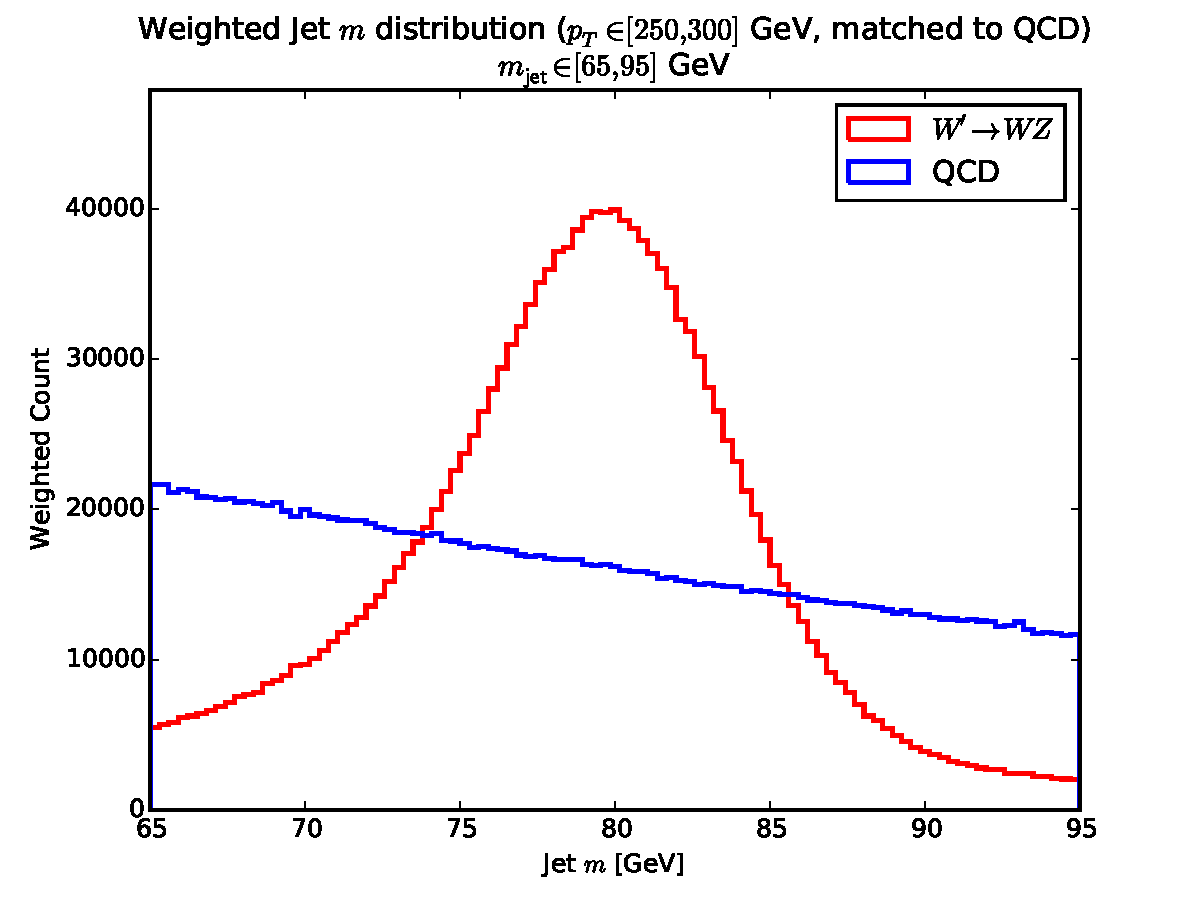
\includegraphics[width=0.5\textwidth]{figures/weighted-mass-distribution[250-300].pdf}
      }
      \subfloat[Weighted $\tau_{21}$ distribution \label{subfig:weighted_nsj}]{
        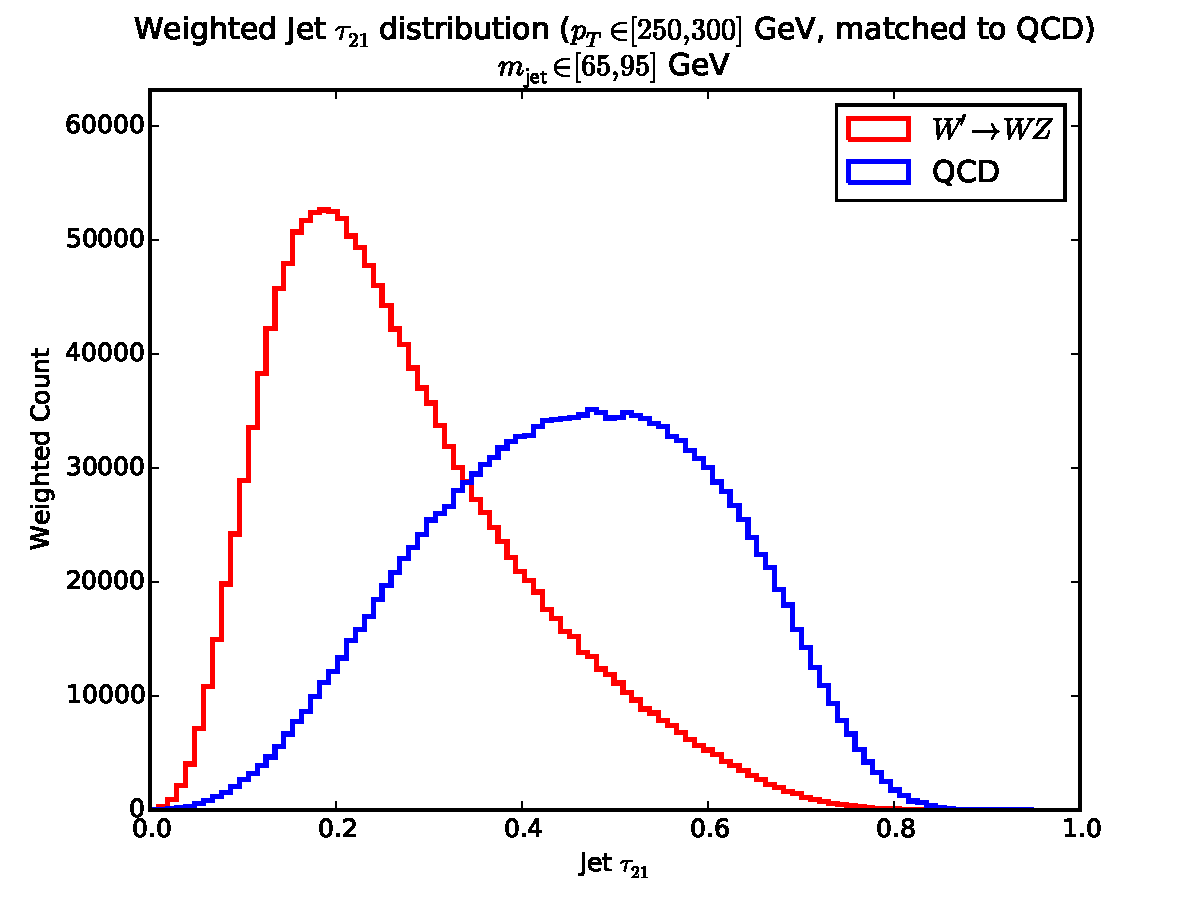
\includegraphics[width=0.5\textwidth]{figures/weighted-tau21-distribution[250-300].pdf}
      }
      \caption{Weighted mass (left) and $n$-subjettiness (right) of samples, with $W'\rightarrow WZ$ decays in red and QCD jets in blue.\label{fig:mass_nsj_spectrum} }
    \end{center}
\end{figure}  



\begin{figure}[bt]
  \begin{center}
  
      \subfloat[Average weighted $W'\rightarrow WZ$ image \label{subfig:weighted_sig}]{
        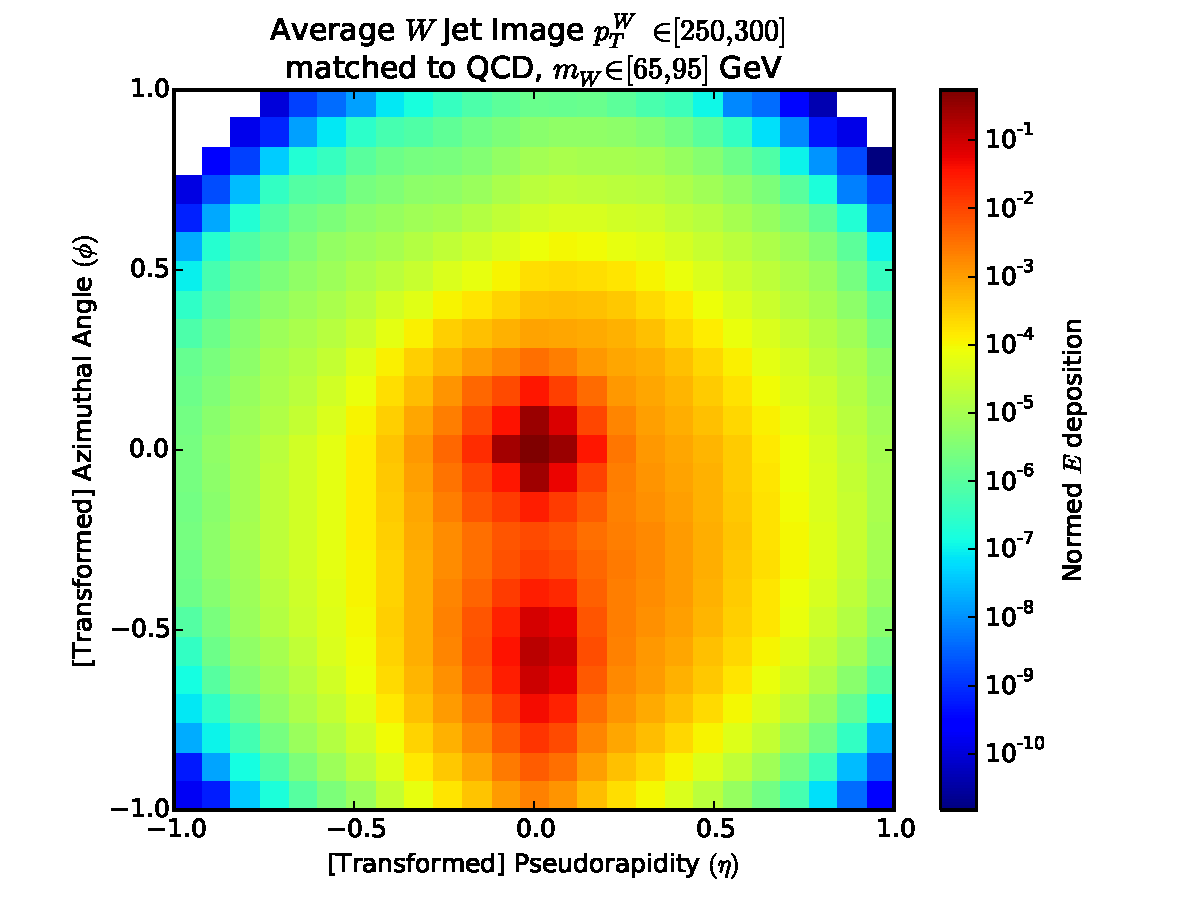
\includegraphics[width=0.5\textwidth]{figures/sig-im.pdf}
      }
      \subfloat[Average weighted QCD image \label{subfig:weighted_bkg}]{
        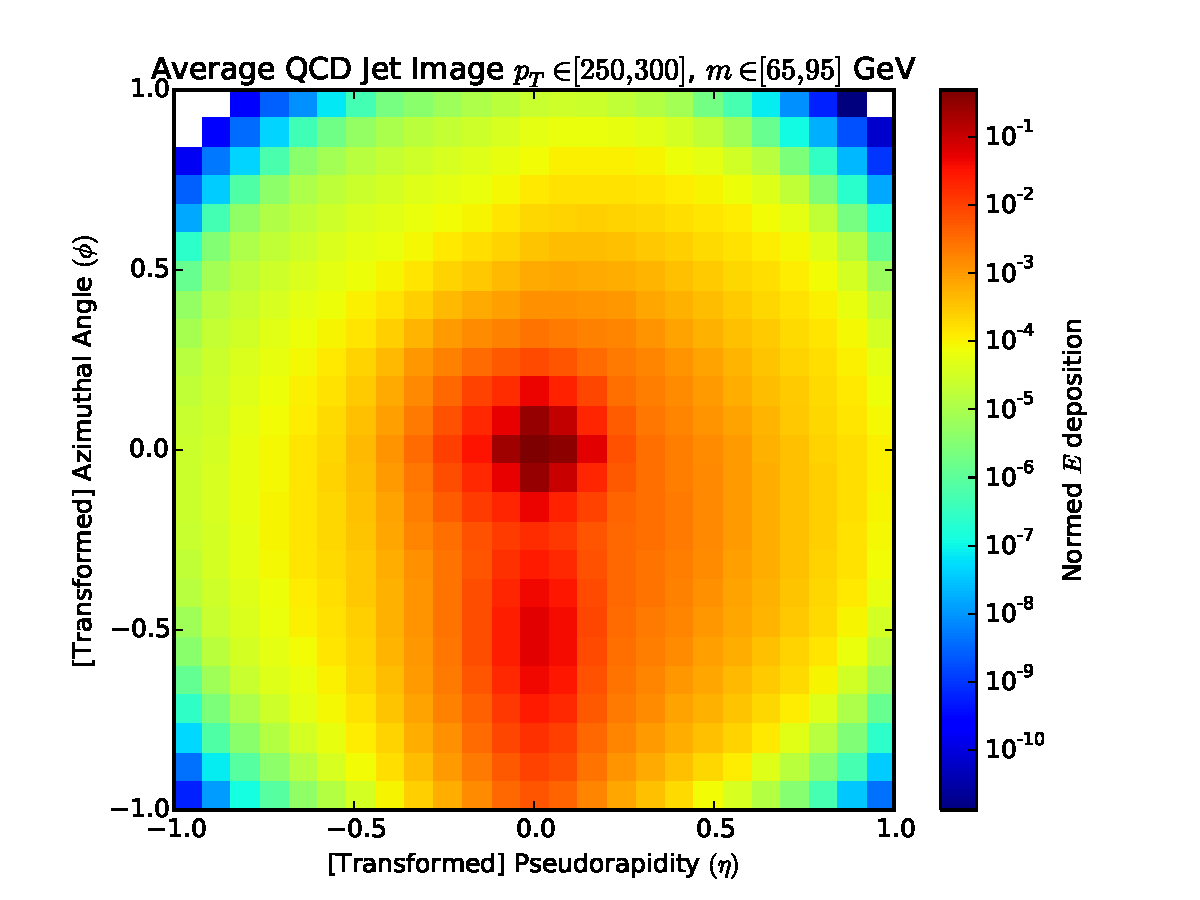
\includegraphics[width=0.5\textwidth]{figures/bkg-im.pdf}
      }
      \caption{Weighted $W'\rightarrow WZ$ (left) and QCD (right) average jet-image
      \label{fig:meanImages} }
    \end{center}
\end{figure}  

Discuss the creation of the jet images.

Discuss the physical differences between W bosons and q/g jets?


%\section{Figure of Merit} % (fold)
\label{sec:figure_of_merit}

As is commonly done in High Energy Physics, we eschew the commonly chosen metric of basic accuracy in favor of the Receiver Operating characteristic. This is because we must examine the entire spectrum of trade-off between Type-I and Type-II error, as many applications in physics will choose different points along the trade-off curve. We use a slight modification of the traditional ROC. For any discriminating variable, let $c$ be a threshold on the likelihood ratio on that variable, and let $w$ be the vector of weights over the entire evaluation sample. We define the \emph{rejection} of such a threshold is defined as 
$$
    \rho(c) = \frac{1}{\text{FPR}(c, w)},
$$
where $\text{FPR}(c, w)$ is the weighted false positive rate for using $c$ as a threshold.

We define the \emph{efficiency} of $c$ as 
$$
    \varepsilon(c) = \text{TPR}(c, w),
$$
where $\text{TPR}(c, w)$ is the weighted false positive rate for using $c$ as a threshold. We then evaluate our algorithms using the area under the line generated by $\{(\varepsilon(c), \rho(c)) : \varepsilon(c)\in [0.2, 0.8]\}$. We say that an classifier is \emph{strictly} more performant if the ROC curve is above a baseline for all efficiencies.

% section figure_of_merit (end)

%\section{Deep Learning} % (fold)
\label{sec:deep_learning}

Since it's first usage by it's current name~\cite{hinton06}, Deep Learning has taken on many forms and seen success in a variety of fields that have traditionally utilized human-engineered features to create classifiers and apply out-of-the-box machine learning algorithms. In particular, the field of Computer Vision has changed drastically. Since the 2012 ILSVRC winning entry by Alex Krizhevsky and the University of Toronto group ~\cite{alexnet}, Deep Learning -- in particular Convolutional Neural Networks -- have taken over vision-based machine learning, consistently showing human and recently super-human levels performance on key baseline datasets. The increasingly widespread availability of GPUs and associated numerical frameworks has made the time intensive estimation procedures associated with deep neural networks more feasible, and has allowed the size of models for image tasks to grow exponentially. For example, the Google team's contribution to ILSVRC 2014 -- the GoogLeNet~\cite{googlenet} -- consisted of 22 layers of convolutional black boxes called ``Inception Units'', and set the benchmarks both for accuracy and speed of a model on such a large scale. 

As it relates to our work, do not investigate large network architectures, rather we focus on  understanding what information and higher level representations a convolutional neural network will learn in the context of High Energy Physics. We let our knowledge of physics guide our investigations into visualization, understanding, and demystification of deep representations for physics. We shed light inside the black-box of deep learning in the context of object identification in HEP.

% section deep_learning (end)

\section{Network Architecture}
\label{sec:arch}

%An in-depth examination of architectures via trial and error is left  future 

We begin with the notion that the discretization procedure outlined in Section \ref{sec:simulation} produces $25\times 25$ ``transverse-energy-scale'' images in one channel -- a High Energy Physics analogue of a grayscale image. We note that the images we work with are \emph{sparse} -- roughly 12\% of pixels are active on average. Future work can build on efficient techniques for exploiting the sparse nature of these images. However, since speed is not our driving force in this work, we used convolution implementations defined for dense inputs.  We also study fully connected MaxOut networks~\cite{maxout:goodfellow}.  Other architectures were also studied, such as Stack Denoising Autoencoders~\cite{SDAE}, and multi-layer fully connected networks with various activation functions, but found that convolution and MaxOut networks were the most performant.

As a brief aside, we discuss some of the key neural network concepts which are used in the following section to describe our network architectures.  Fully connected (FC) layers take all features as input.  Convolution networks utilize convolution filters (or kernels) which are a set of weights $W$ that operate linearly on a small $n\times n$ patch of the input image.  For instance, a $3\times3$ filter takes as input a $3\times3$ (horizontal $\times$ vertical) patch of pixels and outputs $z = \sum_{i,j=1}^{3} x_{ij}W_{ij}$, where $x_{ij}$ is the input image patch.  The filter output can be considered as centered on that patch.  Each filter is convolved with the input image, in that the filter is applied to a given input patch and then moved horizontally and/or vertically to a new input patch on which the filter is applied.  By scanning over the entire image in this way, a the filter is convolved with the input, producing a convolved output. An important consideration when considering convolutional networks is how one handles borders of images. Two main options exist -- one can only consider $n\times n$ patches that are fully contained within the input images, or one can consider every convolution that has at least one pixel from the image, \emph{zero-padding} as necessary to create valid convoltutions. We use the latter, as we found better performance and better, more physics-driven filters. 

A non-linear activation function is typically applied to these convolution outputs, for which we use the Rectified Linear Unit (ReLU)~\cite{RELU} that takes an input $z$ and outputs $\max\{0,z\}$. ReLU's have been found to improve network training time, whilst having enough non-linear behavior to not degrade network performance. In addition, Rectified Linear Units do not suffer from a vanishing gradient, and speed up computation time while allowing for sparse networks by having true zero-valued activations.  After convolution(+activation) layers, a non-linear down-sampling is frequently performed using Max-pooling~\cite{MAXPOOL} which takes non-overlapping patches of convolution outputs as input, and outputs the maximum value for each patch.  Finally, the MaxOut network makes use of the Dense (Fully Connected) MaxOut activation unit, which takes an input vector $x$ and computes $k$ linear weightings $z_{j\in [1,k]} = \sum_{i} x_{i} W_{ij} + b_{j}$ and  outputs $\max_{j\in [1,k]}\ z_{j}$. Natural extensions of MaxOut layers to convolutional units exist, but were not examined. Conceptually, one can view the Rectified Linear Unit as a special case of the MaxOut with $k=2$ and one of the layers forced to output only zero. Though MaxOut units do not force sparsity in the same way as ReLU units, MaxOut networks provide many desirable effects in that they pair nicely with the model averaging effects of dropout in a natural way~\cite{maxout:goodfellow}. 

\subsection{Architectural Selection} % (fold)
\label{ssub:architectural_selection}
For the MaxOut architecture, we utilize two FC layers with MaxOut activation (the first with 256 units, the second with 128 units, both of which have 5 piecewise components in the MaxOut-operation), followed by two FC layers with ReLU activations (the first with 64 units, the second with 25 units), followed by a FC sigmoid layer for classification. We found that the He-uniform initialization~\cite{HE_initialization} for the initial MaxOut layer weights was needed in order to train the network, which we suspect is due to the sparsity of the jet-image input. In cases where other initialization schemes were used, the networks often converged to very sub optimal solutions.  This network is trained (and evaluated) on un-normalized jet-images using the transverse energy for the pixel intensities

For the deep convolution networks, we use a convolutional architecture consisting of three sequential \texttt{[Conv + Max-Pool + Dropout]} units, followed by a local response normalization (LRN) layer~\cite{dropout:and:LRN}, followed by two fully connected, dense layers. We note that the convolutional layers used are so called ``full'' convolutions -- i.e., zero padding is added the the input pre-convolution. A conceptual visualization of the network architecture can be seen in Figure~\ref{fig:arch}. Our architecture can be succinctly written as:
\begin{equation}
  \mathtt{[Dropout \rightarrow Conv \rightarrow ReLU \rightarrow MaxPool] * 3 \rightarrow LRN \rightarrow [Dropout \rightarrow FC \rightarrow ReLU]  \rightarrow Dropout \rightarrow Sigmoid}.
\end{equation}

\begin{figure}[!htbp]
  \centering
  \includegraphics[width=0.75\textwidth]{figures/architecture.pdf}
  \caption{The convolution neural network concept as applied to jet-images.}
  \label{fig:arch}
\end{figure}

The convolution layers each utilize 32 feature maps, or filters, with filter sizes of $11\times 11$, $3\times 3$, and $3\times 3$ respectively.  All convolution layers are regularized with the $L^{2}$ weight matrix norm.  A down-sampling of $(2, 2)$, $(3, 3)$, and $(3, 3)$ is performed by the three max pooling layers, respectively.  A dropout~\cite{dropout:and:LRN} of 20\% is used before the first FC layer, and a dropout 10\% is used before the output layer.  The FC hidden layer consists of 64 units.

After early experiments with the standard $3\times 3$ filter size, we discovered significantly worse performance over a more basic MaxOut \cite{maxout:goodfellow} feedforward network. After further investigation into larger convolutional filter size, we discovered that larger-than-normal filters work well on our application. Though not common in the Deep Learning community, we hypothesize that this larger filter size is helpful when dealing with sparse structures in the input images. In Table~\ref{tab:kernelsize}, we show the optimal filter size of $11\times11$ while considering the metric outlined in Section~\ref{sec:studies}.

\begin{table}[h!]
  \centering
  \begin{tabular}{r|c}
    \bfseries Kernel size & \bfseries AUC \\ 
    \hline
    $(3 \times 3)$ Conv & 14.770 \\
    \hline
    $(4 \times 4)$ Conv & 12.452 \\
    \hline
    $(5 \times 5)$ Conv & 11.061 \\
    \hline
    $(7 \times 7)$ Conv & 13.308 \\
    \hline
    $(9 \times 9)$ Conv & 17.291 \\
    \hline
    $(11 \times 11)$ Conv & 20.286 \\
    \hline
    $(15 \times 15)$ Conv & 18.140 \\
  \end{tabular}
  \caption{First layer convolution size vs. performance}
  \label{tab:kernelsize}
\end{table}
% table

Two convolution networks, which differ in their pre-processing, are studied in this paper.  The first, which we refer to as the ConvNet, is trained (and evaluated) on un-normalized jet-images using the transverse energy for the pixel intensities.  The second, which we refer to as ConvNet-Norm, is trained (and evaluated) on $L^{2}$ normalized jet-images using the transverse-energy for the pixel intensities.  Examining the performance of both networks allows us to study the possible effects of the pre-processing.



% subsubsection architectural_selection (end)

\subsection{Implementation and Training} % (fold)
\label{ssub:implementation_and_training}

All Deep Learning experiments were conducted in Python with the Keras~\cite{Keras} Deep Learning library, utilizing NVIDIA C2070 graphics cards. One GPU was used per training, but several architectures were trained in parallel on different GPU's to optimize the performance of networks with different hyper-parameters.

We used 8 million training examples, with an additional 2 million validation samples for tuning the hyper-parameters, and 3 million testing samples.  Signal examples are weighted such that the total sum of weights is the same as the total number of background examples (as explained in Section~\ref{sec:simulation}).  These weights are used in the by the cost function in the training.  The networks were trained with the Adam~\cite{DBLP:journals/corr/KingmaB14} algorithm (Stochastic Gradient Descent with Nesterov Momentum~\cite{Nesterov:1983wy} was also examined, but did not provide performance gains).  The training consisted of 100 epochs, with a 10 epoch patience parameter on the increase in AUC between 0.2 and 0.8 on a validation set.  Batch sizes of 32 were used for the MaxOut network, while batch sizes of 96 were used for the convolution networks.

% subsubsection implementation_and_training (end)



\section{Studies} % (fold)
\label{sec:studies}

To begin understanding what a deep network can learn about jet topology, we choose a finite region of phase space, and standardize our comparisons. In an effort to define a standard way that physics object identification using machine learning should be conducted, we exactly define our procedure for comparisons. In particular, we restrict our studies to $250$ GeV $\leq p_T \leq 300$ GeV, and confine ourselves to a $65$ GeV $\leq m \leq 95$ GeV mass window, wholly containing the peak of the $W$. 

We construct a scaffolded and multi-approach series of methodologies for understanding, visualizing, and validating neural networks within HEP.

\subsection{Coarse Studies} % (fold)
\label{sub:coarse_studies}

To a first order, the first desirable characteristic is a simple performance improvement over the standard physics-driven variables for discrimination. In particular, we compare our network to $n$-subjettiness~\cite{nsub} and the jet mass. We henceforth refer to $n$-subjettiness as $\tau_{21}$ for our purposes, as $\tau_{2}/\tau_{1}$ is relevant for our classification problem.

In Figure~\ref{fig:combinedROC}, we illustrate the performance gains of a deep neural network over both $\tau_{21}$ and the 2D likelihood of $\tau_{21}$ and jet mass. 


\begin{figure}[!htbp]
  \centering
  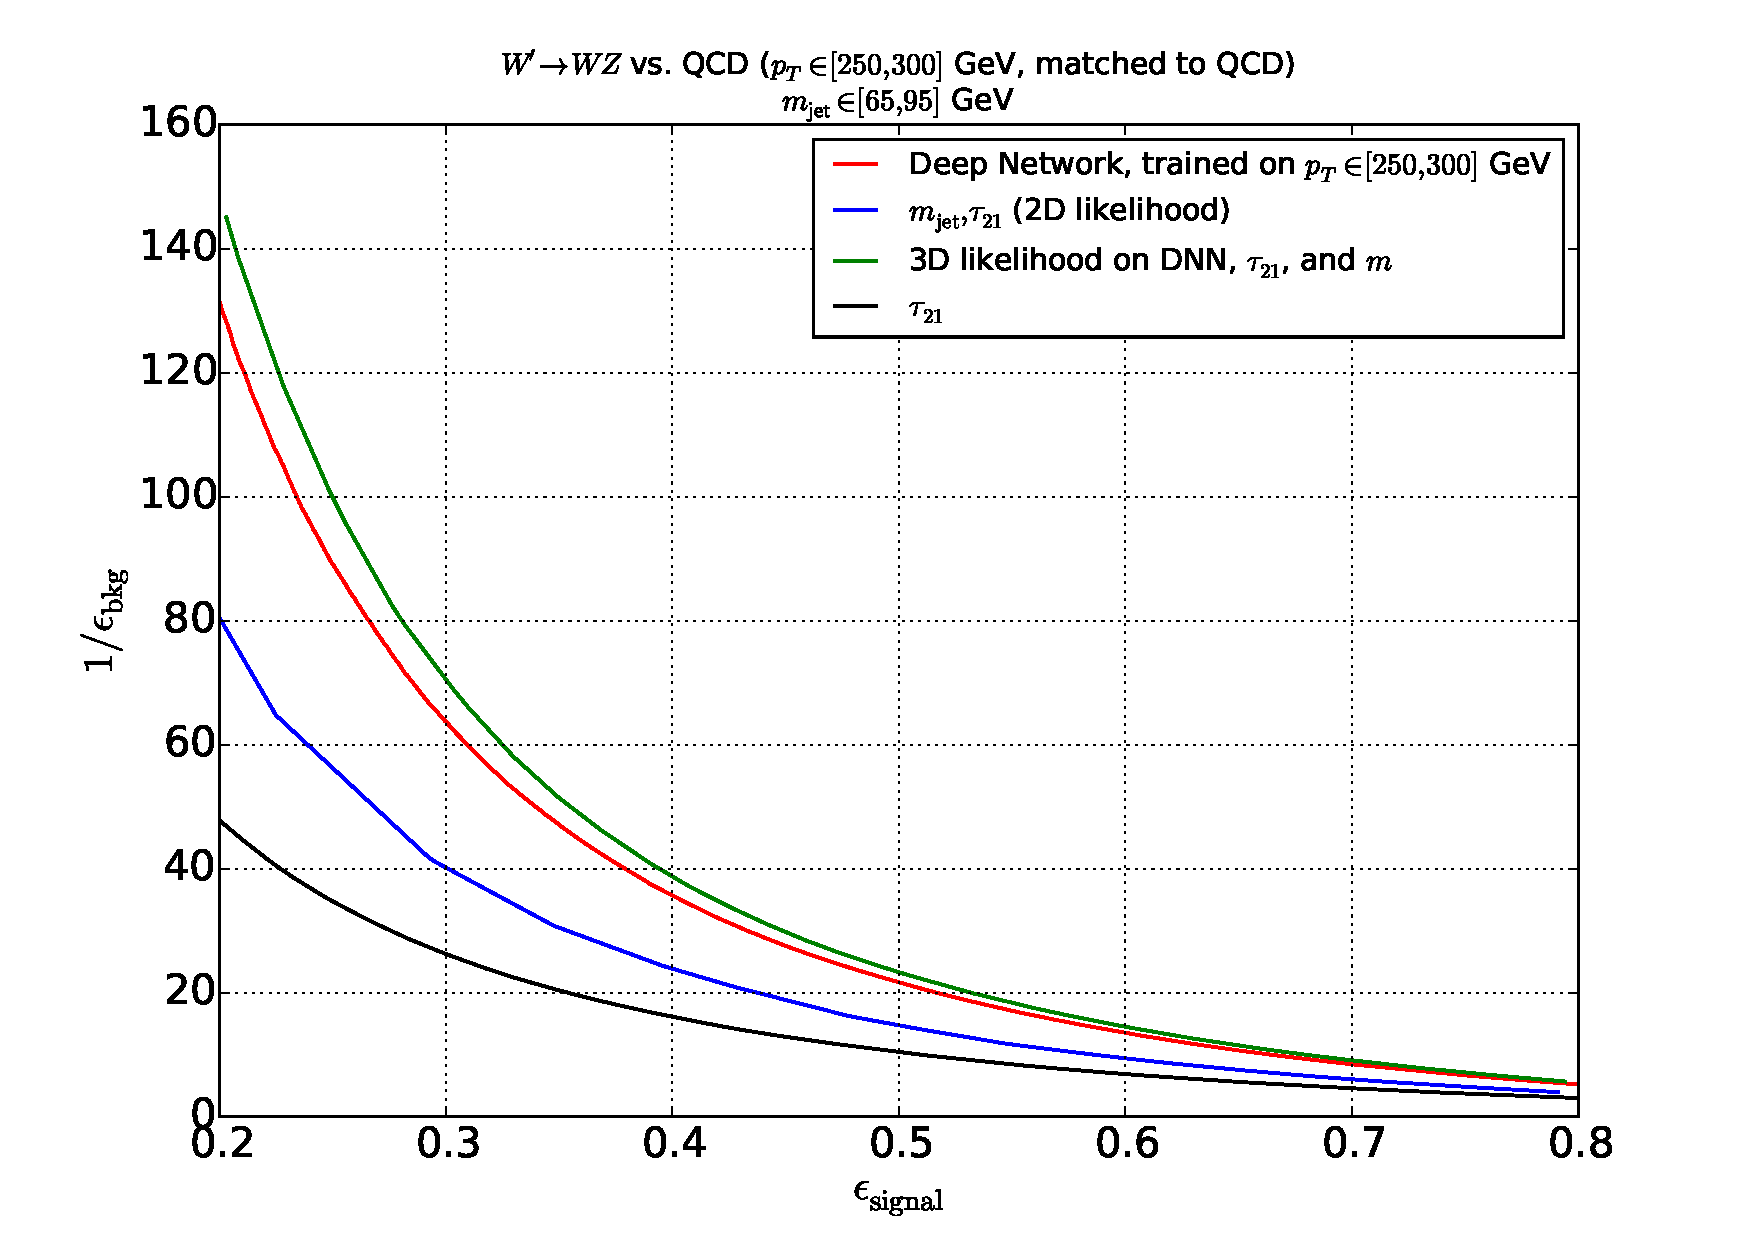
\includegraphics[width=0.95\textwidth]{figures/combined-roc.pdf}
  \caption{Receiver Operating Characteristic (ROC) over coarse sample}
  \label{fig:combinedROC}
\end{figure}

We also provide a comparison to a 3D likelihood constructed on $\tau_{21}$, jet mass, and the deep network output itself. We can gain a significant piece of insight from this. Note how in Figure~\ref{fig:combinedROC} we can see that the DNN represents a large gain on a physics-only likelihood. However, when we explicitly include the physics variable in a 3D likelihood, we see a small but definitively non-zero performance gain. This implies that the performance boost \emph{by definition} is getting its gain from something that is not \emph{fully} encapsulated in $\tau_{21}$ and jet mass. 

Though important on it's own, this figure of merit does little to help drive understanding in the context of HEP. Such an increase begs further questions -- what is this gain, and where does it come from? Why is the DNN able to pick up on this?



\subsubsection{Understanding what is learned} % (fold)
\label{ssub:understanding_what_is_learned}

% subsubsection understanding_what_is_learned (end)
In Figure~\ref{fig:convkernels}, we first examine the $11\times11$ convolutional filters in the first layer and look for structure. In

In order to understand what we learn, we first take a look \emph{inside} the deep network. 
\begin{figure}[bt]
  \begin{center}
      \subfloat[$(11\times11)$ convolutional kernels from first layer \label{subfig:filters}]{
        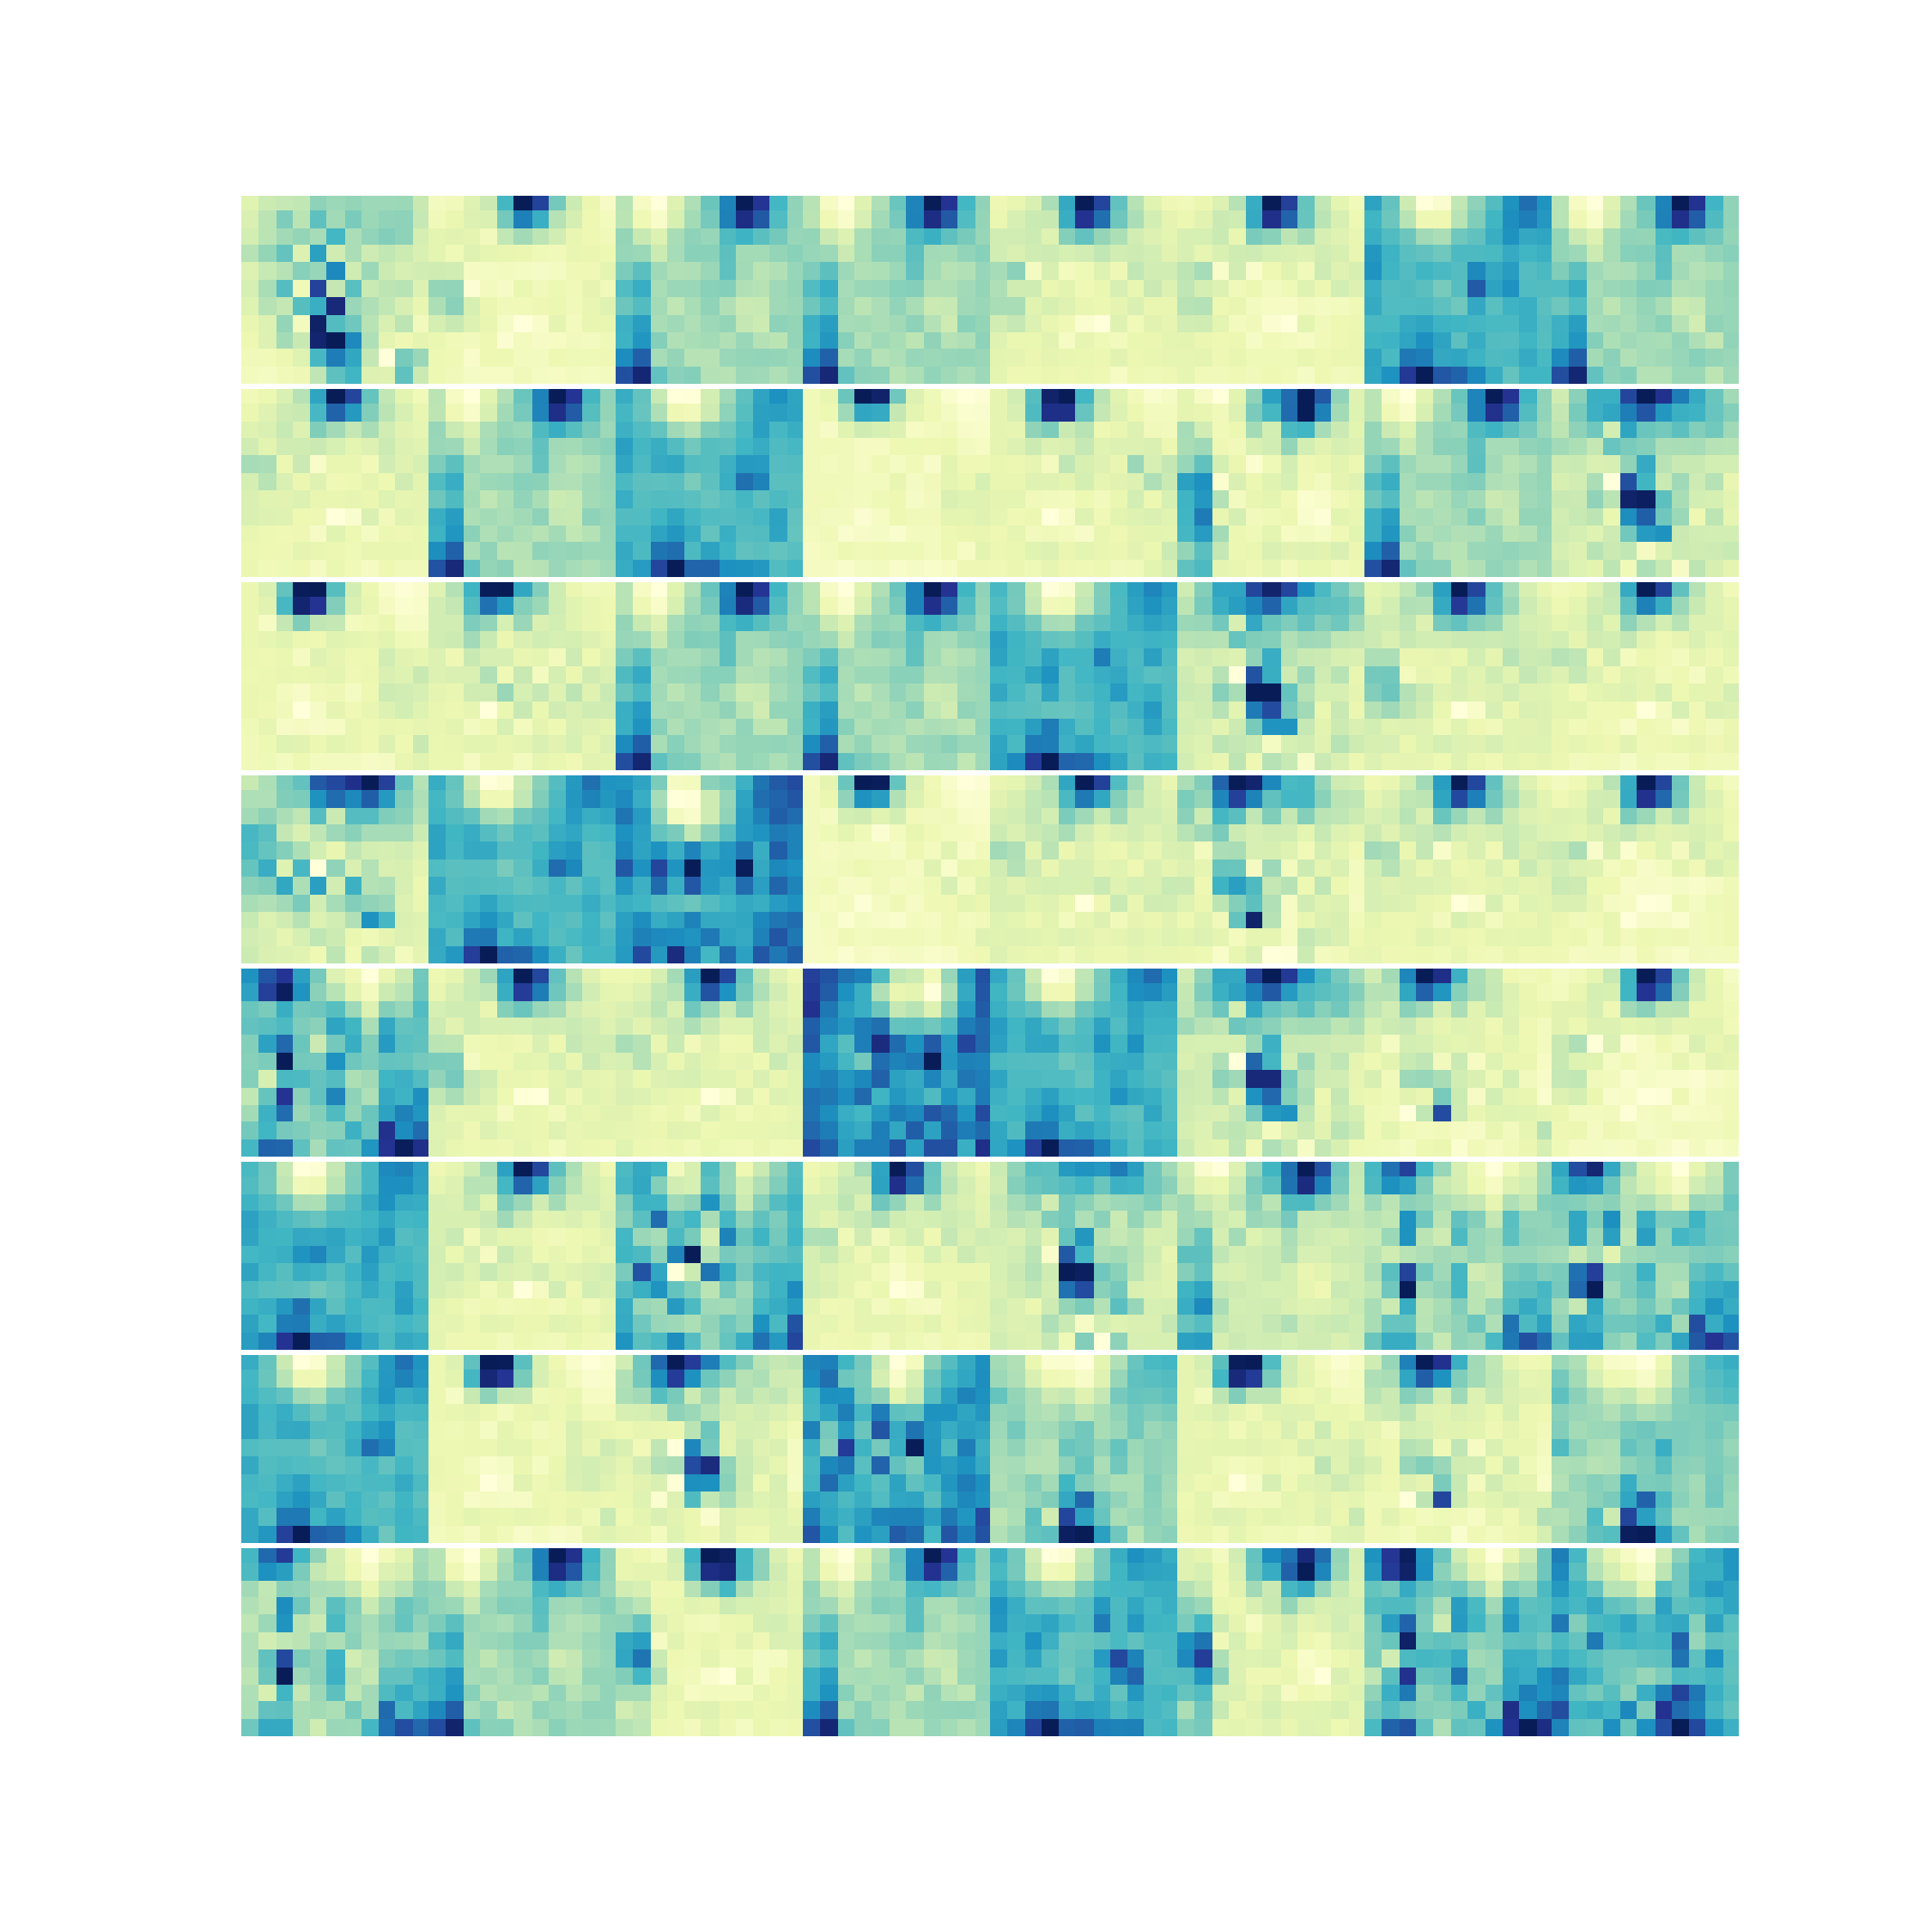
\includegraphics[width=0.5\textwidth]{figures/conv-filts.pdf}
      }
      \subfloat[Convolved Jet Image differences\label{subfig:convolvedfilters}]{
        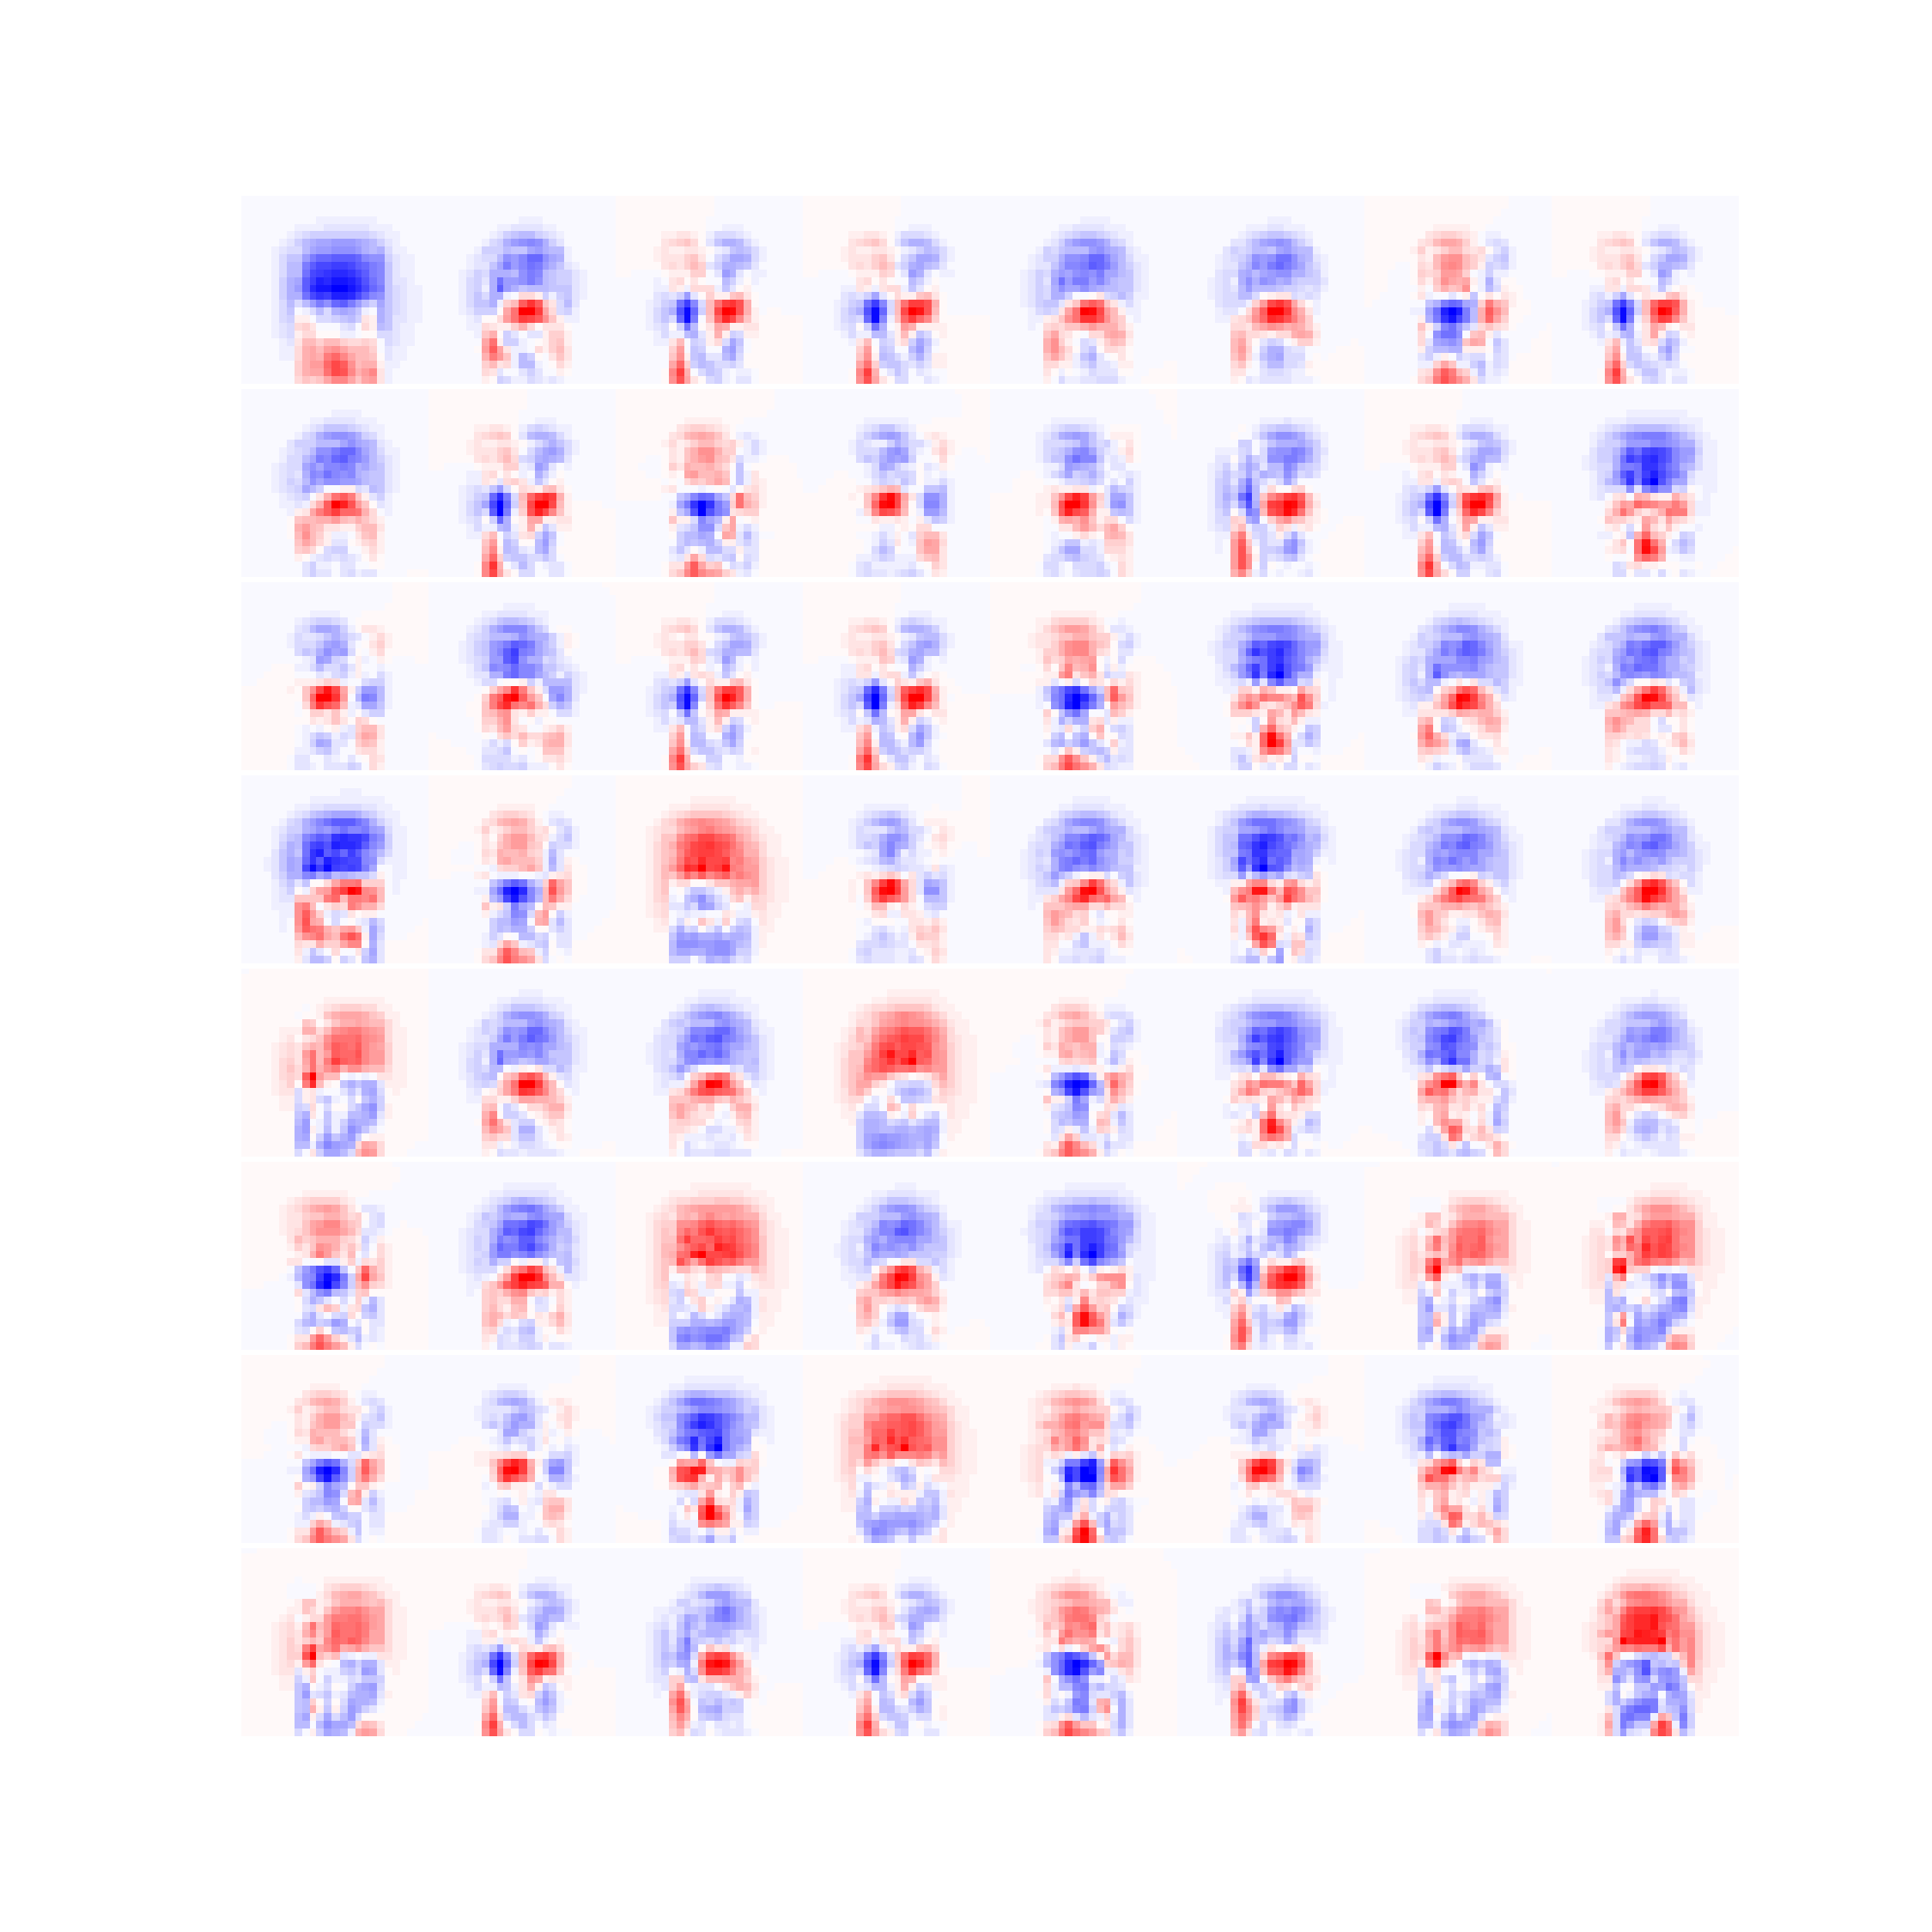
\includegraphics[width=0.5\textwidth]{figures/conv-diffs-global.pdf}
      }
      \caption{Convolutional Kernels (left), and convolved feature differences in jet images (right)}
      \label{fig:convkernels}

    \end{center}
\end{figure}



Blah... linear correlations with pixels





\subsubsection{Physics in Deep Representations} % (fold)
\label{ssub:physics_in_deep_representations}


\begin{figure}[!htbp]
  \centering
  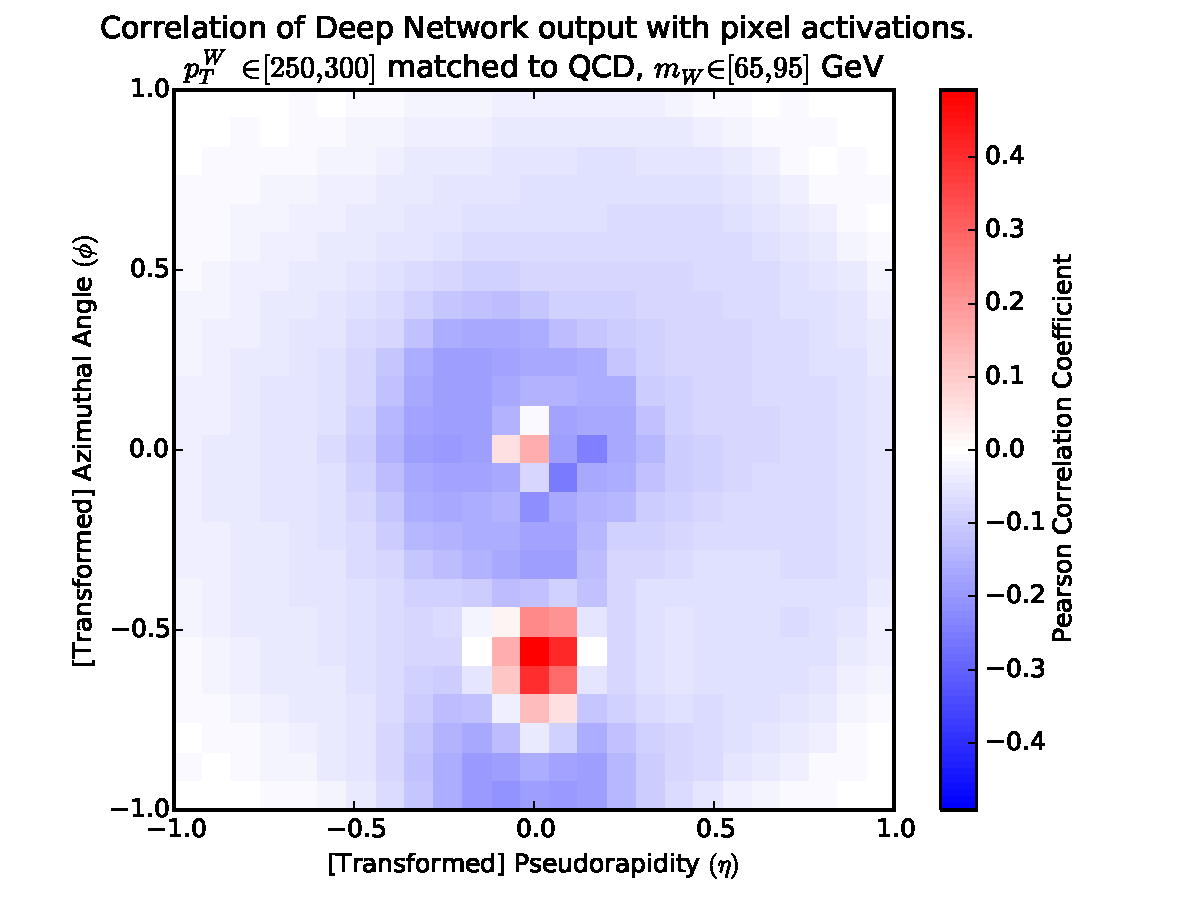
\includegraphics[width=0.95\textwidth]{figures/pixel-activations-corr.pdf}
  \caption{Per-pixel linear correlation with DNN output}
  \label{fig:corr}
\end{figure}


\begin{figure}[bt]
  \begin{center}
      \subfloat[Sculpted QCD $\Delta R$ distribution\label{fig:sculpteddR}]
      {
        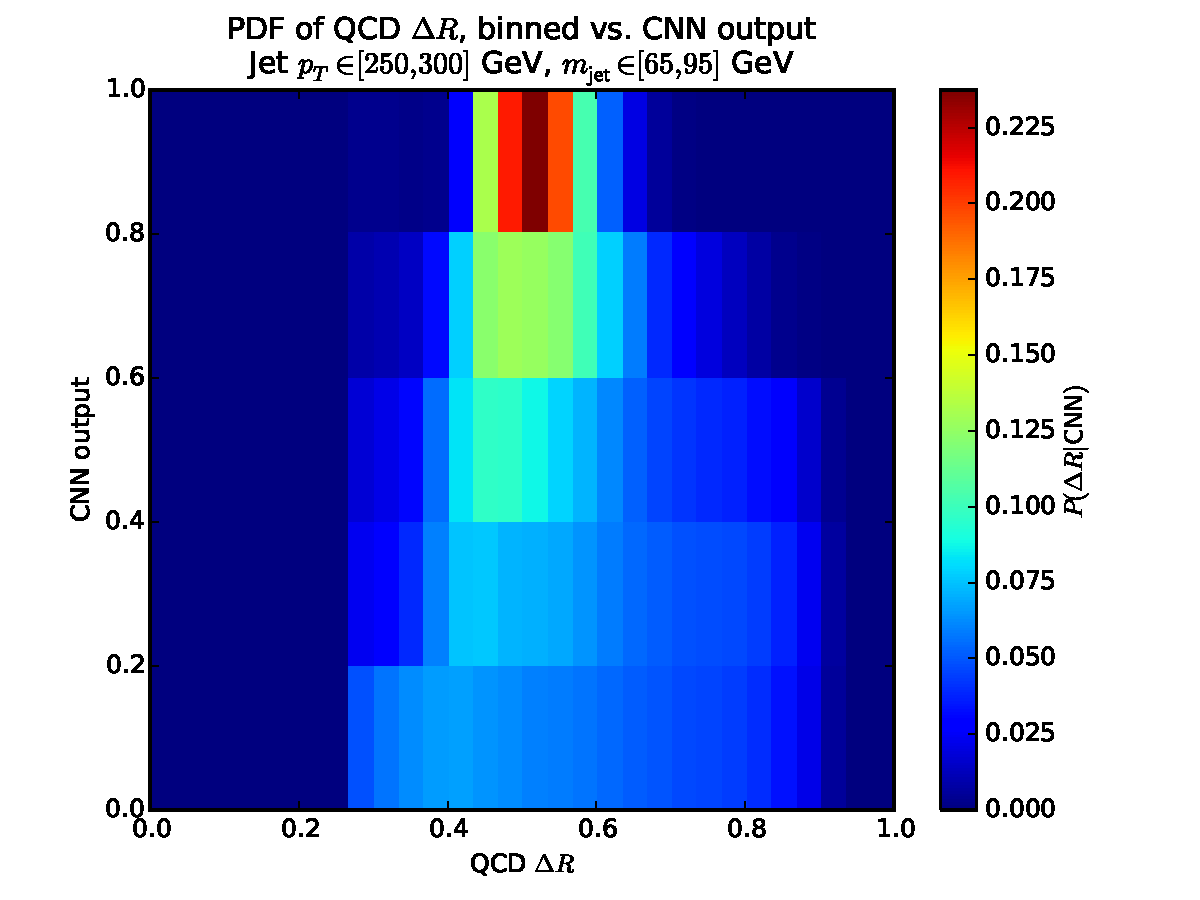
\includegraphics[width=0.5\textwidth]{figures/dR-dist-by-CNN.pdf}
      }
      \subfloat[Sculpted QCD $\tau_{21}$ distribution\label{fig:sculptednsj}]
      {
        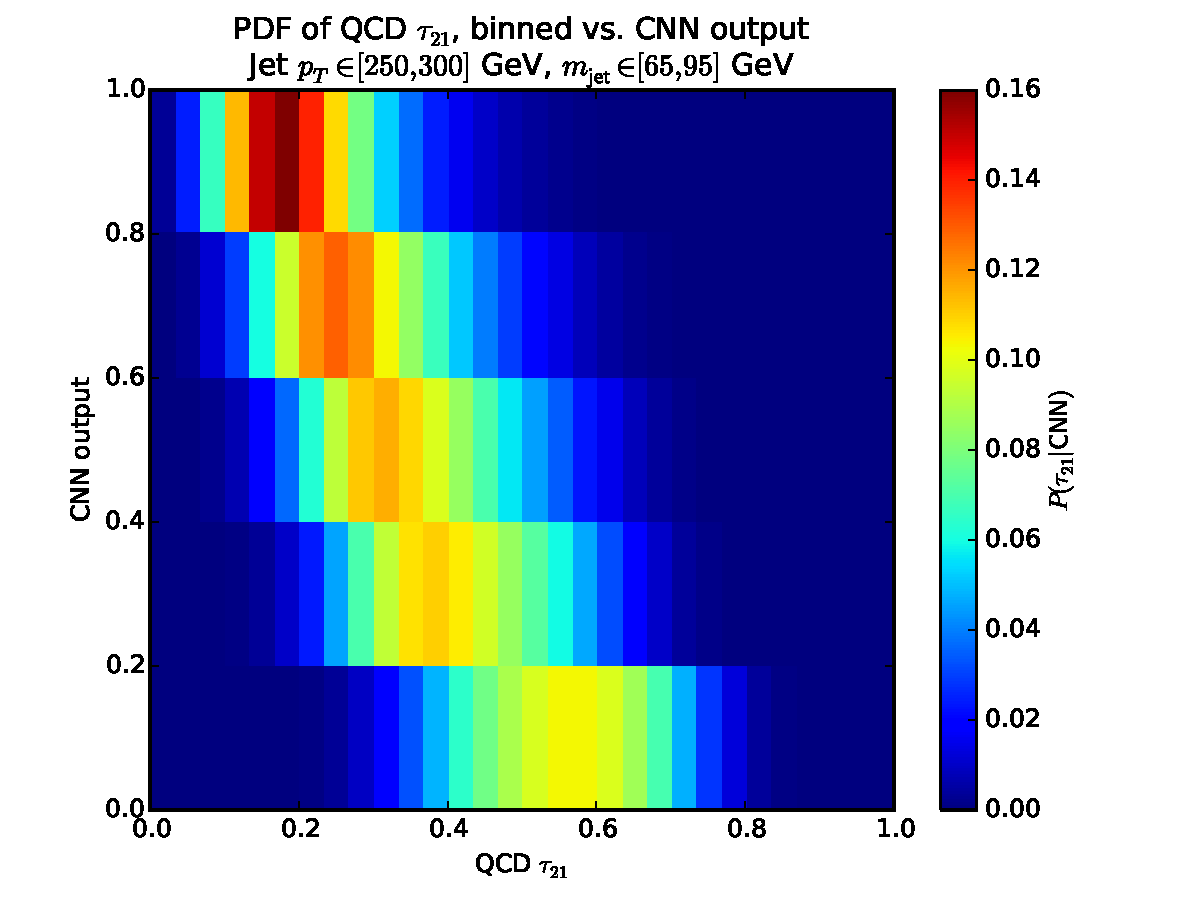
\includegraphics[width=0.5\textwidth]{figures/tau-dist-by-CNN.pdf}
      }
      \\
      \subfloat[Sculpted QCD mass distribution\label{fig:sculptedmass}]
      {
        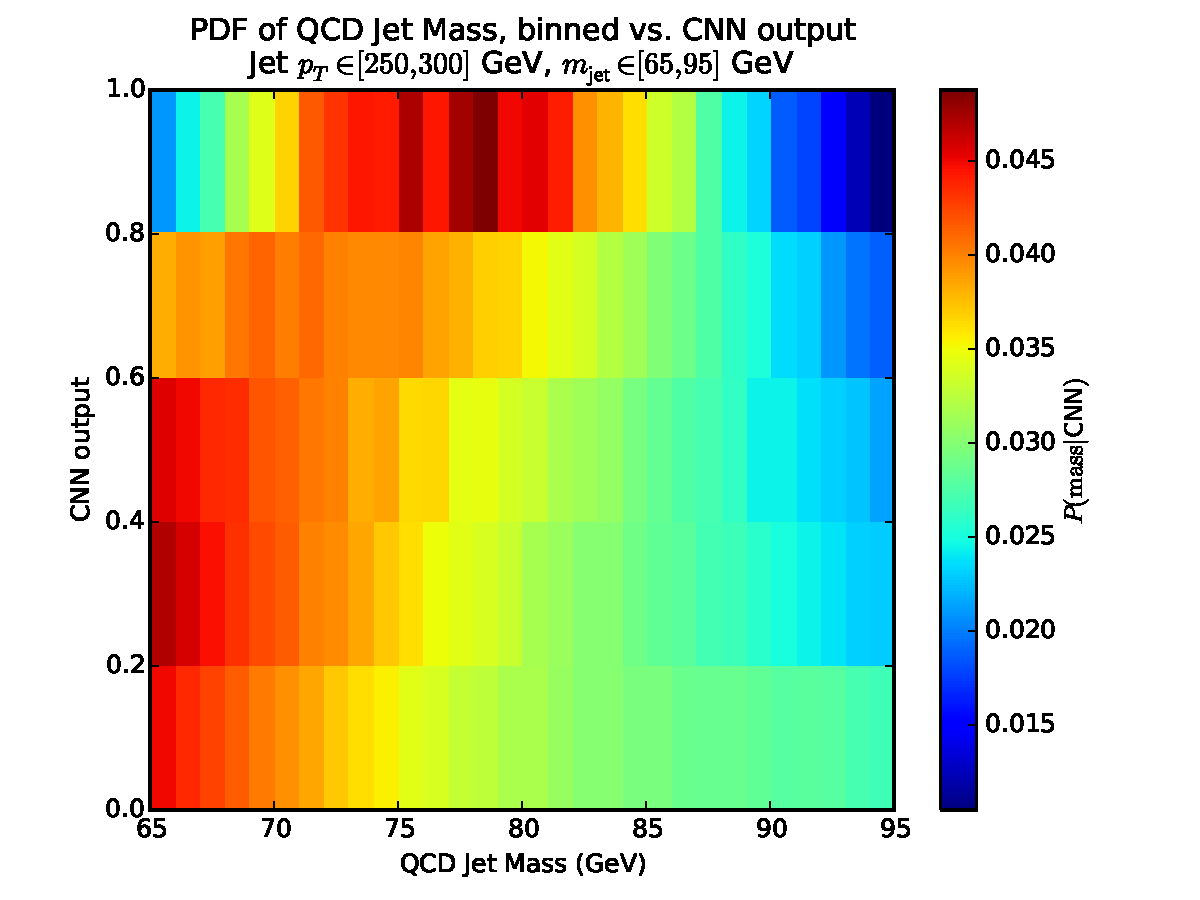
\includegraphics[width=0.5\textwidth]{figures/mass-dist-by-CNN.pdf}
      }

      \caption{Sculpted QCD distributions}
      \label{fig:qcdsculpt}

    \end{center}
\end{figure}





% subsubsection physics_in_deep_representations (end)

% subsection coarse_studies (end)

\subsection{Flat Hypercube Studies} % (fold)
\label{sub:flat_hypercube_studies}


Here, we see the ROC blah...

\begin{figure}[htbp]
  \centering
  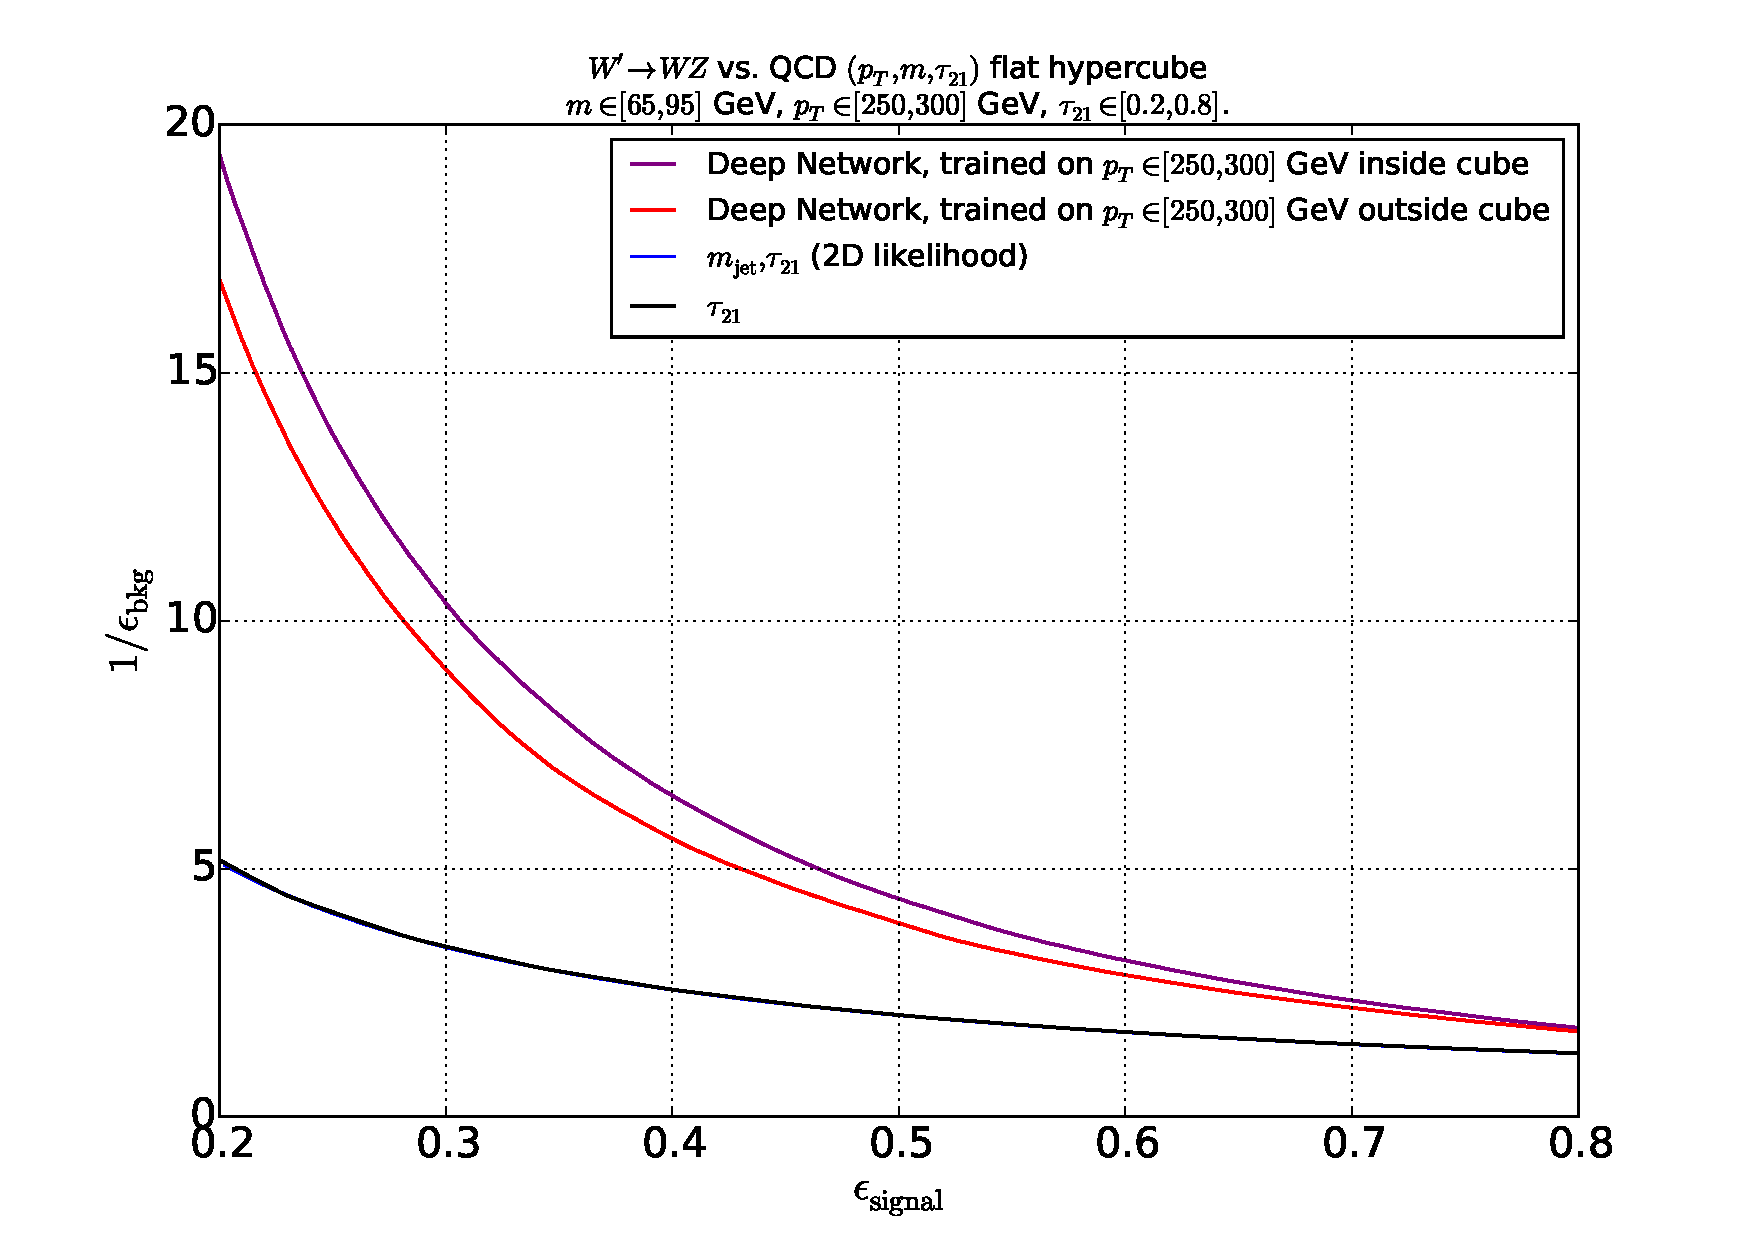
\includegraphics[width=0.95\textwidth]{figures/roc-cube-inside.pdf}
  \caption{ROC Curve for weigth-flattened hypercube, with $m\in[65, 95]\mathsf{GeV}$,  $p_T\in[250, 300]\mathsf{GeV}$, and  $\tau_{21}\in[0.2, 0.8]$}
  \label{fig:rocCube}
\end{figure}

% subsection flat_hypercube_studies (end)



\subsection{Small Window Studies} % (fold)
\label{sub:small_window_studies}


\begin{figure}[bt]
  \begin{center}
  
      \subfloat[Average $W'\rightarrow WZ$ image \label{subfig:sig_window}]{
        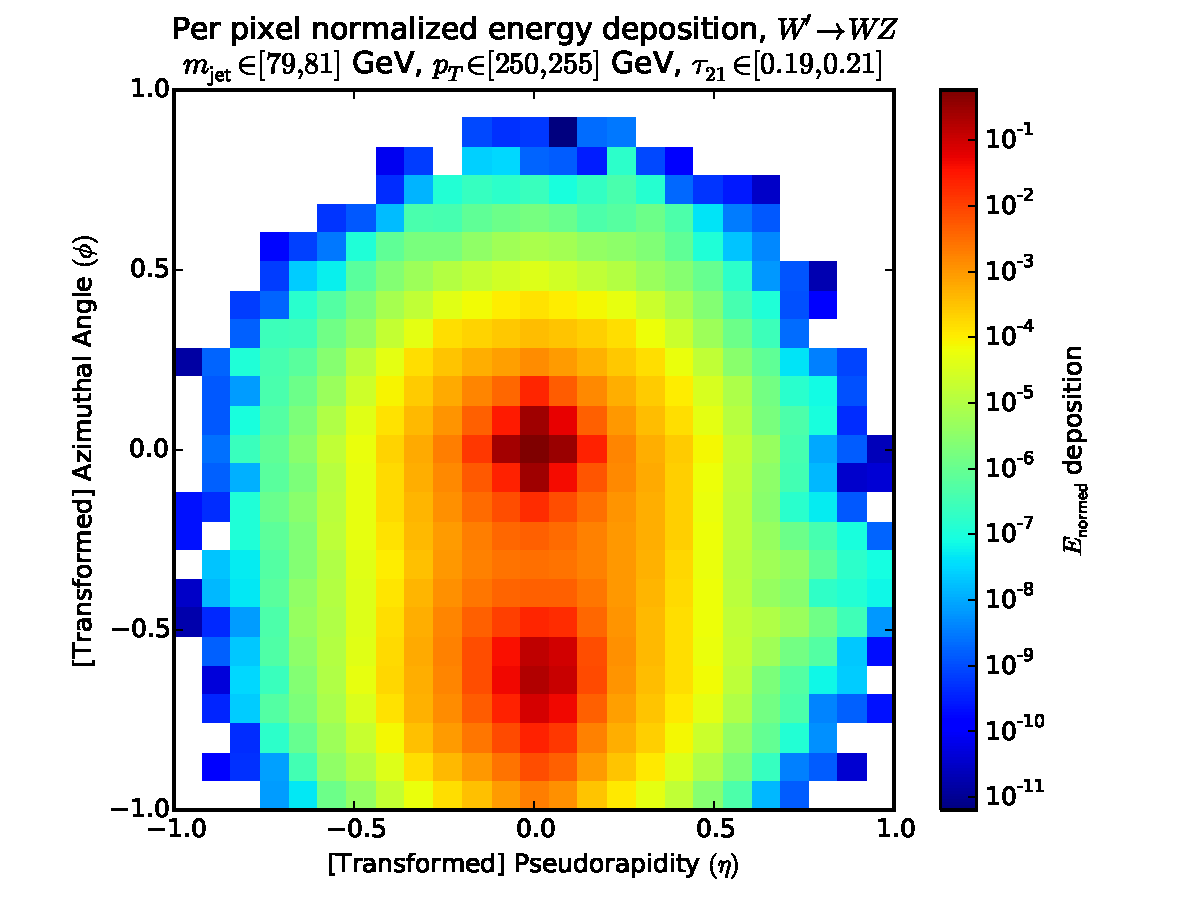
\includegraphics[width=0.5\textwidth]{figures/avg-benwindow-sig.pdf}
      }
      \subfloat[Average QCD image \label{subfig:bkg_window}]{
        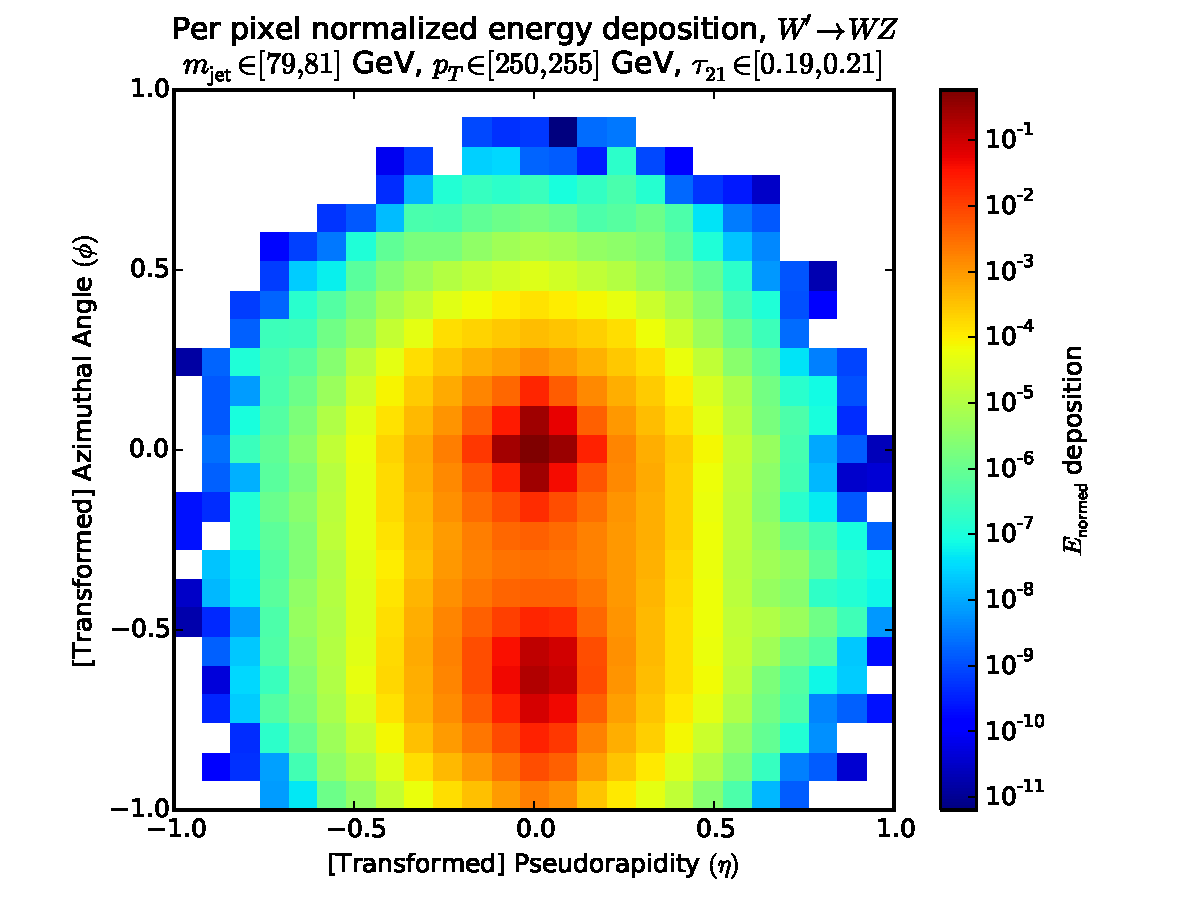
\includegraphics[width=0.5\textwidth]{figures/avg-benwindow-sig.pdf}
      } \\
      \subfloat[Average image difference \label{subfig:windowdiff}]{
        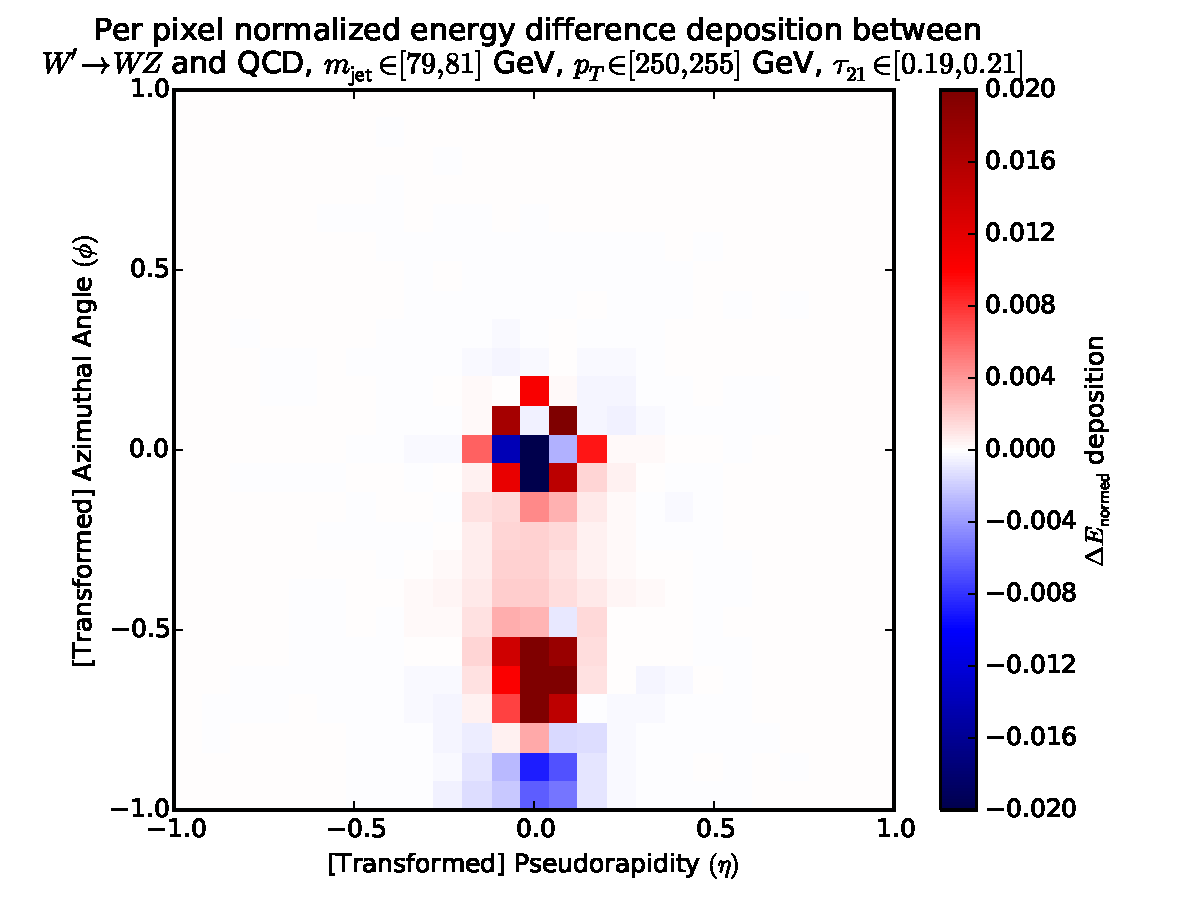
\includegraphics[width=0.5\textwidth]{figures/avg-benwindow-diff-clipped.pdf}
      }
      \caption{$W'\rightarrow WZ$ (left) and QCD (right) average jet-images, and Signal - Background image difference (bottom)
      \label{fig:meanImagesWindow} }
    \end{center}
\end{figure}  


Performance inside the window, use a Fisher Discriminant...

\begin{figure}[htbp]
  \centering
  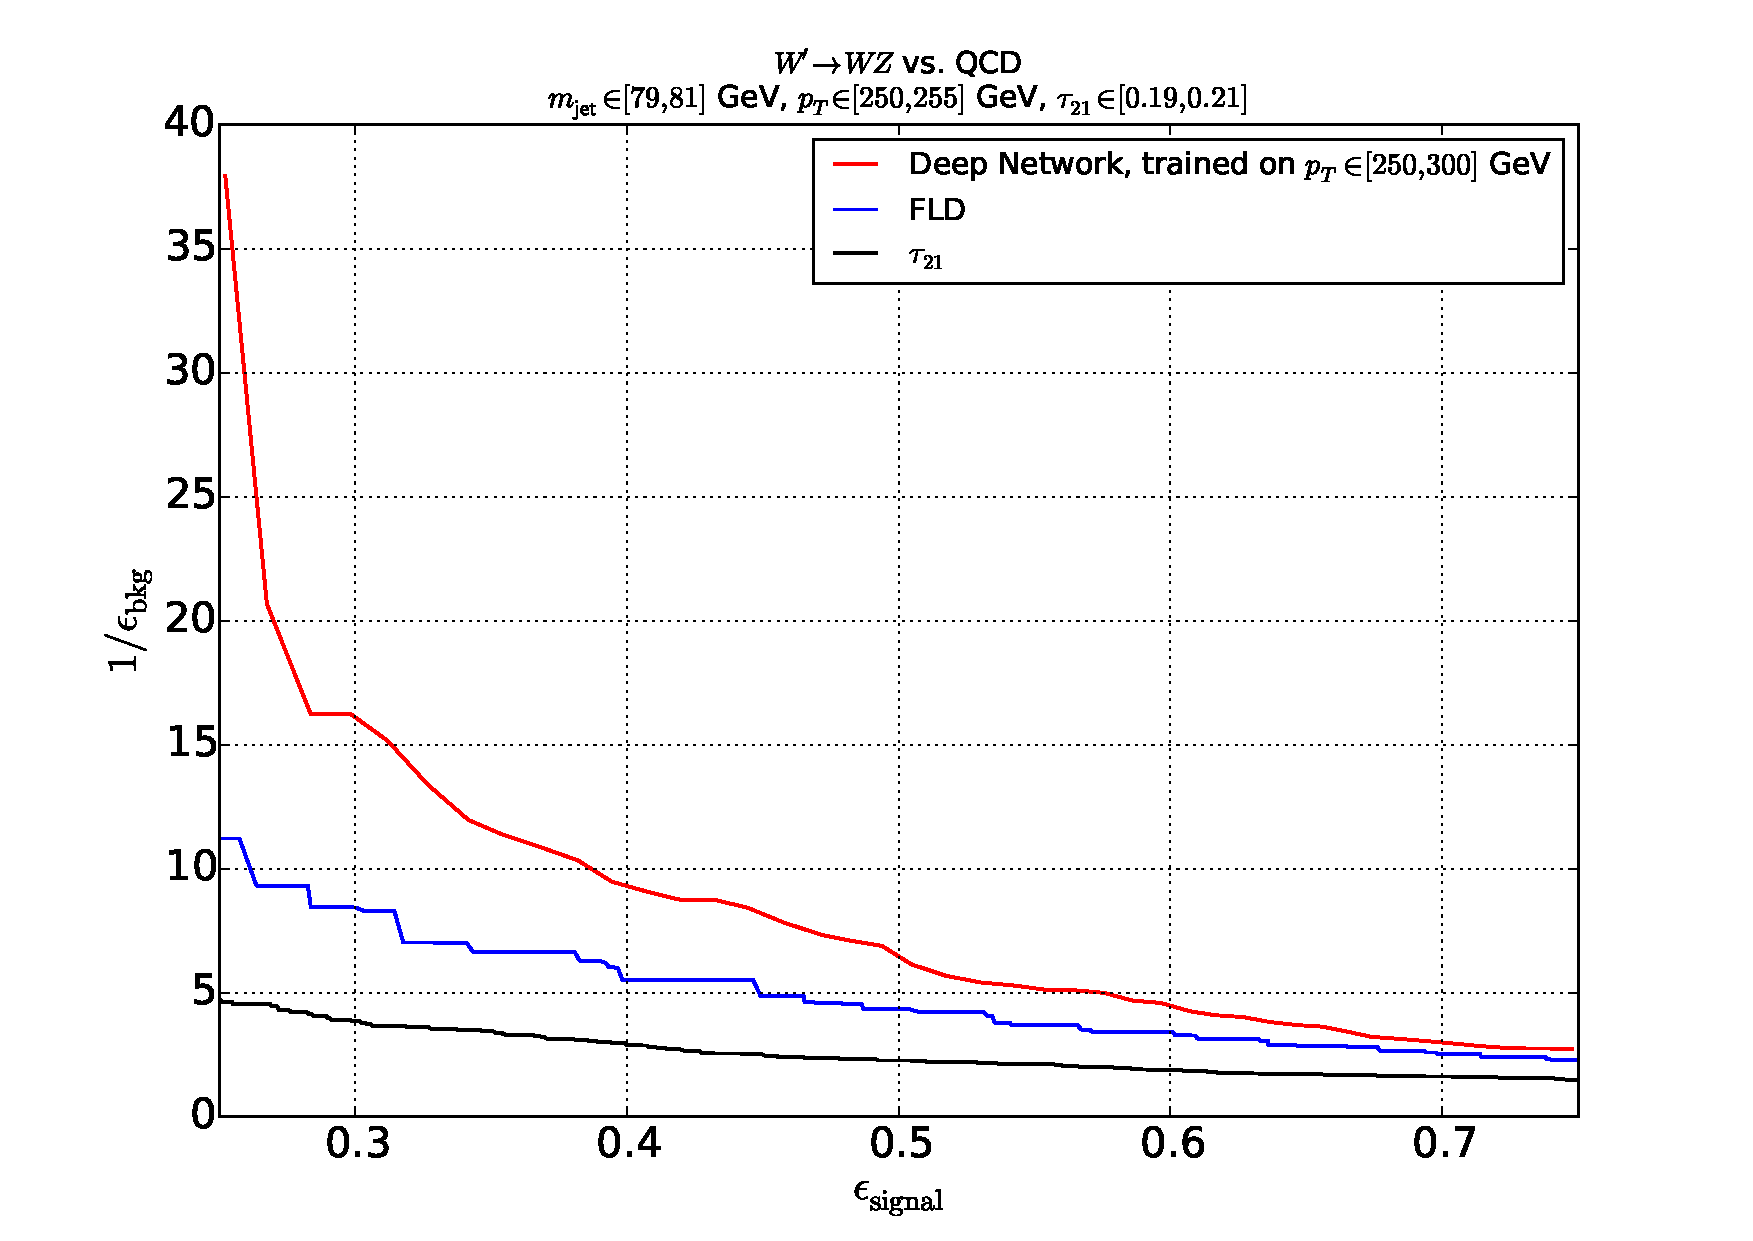
\includegraphics[width=0.95\textwidth]{figures/augwindow-roc.pdf}
  \caption{Receiver Operating Characteristic (ROC) over window sample}
  \label{fig:rocWindow}
\end{figure}

\subsubsection{Understanding what we learn} % (fold)
\label{ssub:understanding_what_we_learn}

\begin{figure}[htbp]
  \centering
  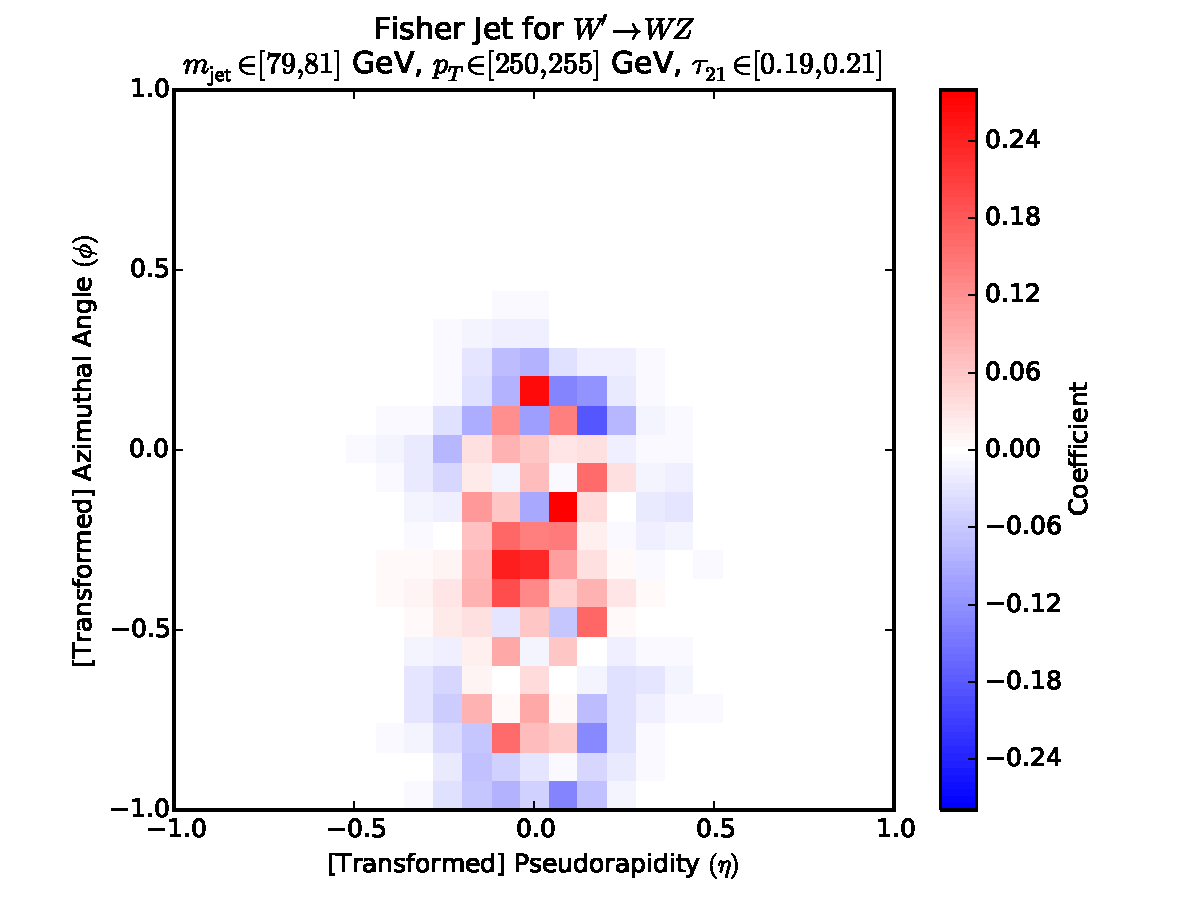
\includegraphics[width=0.65\textwidth]{figures/fld-benwindow.pdf}
  \caption{caption}
  \label{fig:fldWindow}
\end{figure}

\begin{figure}[htbp]
  \centering
  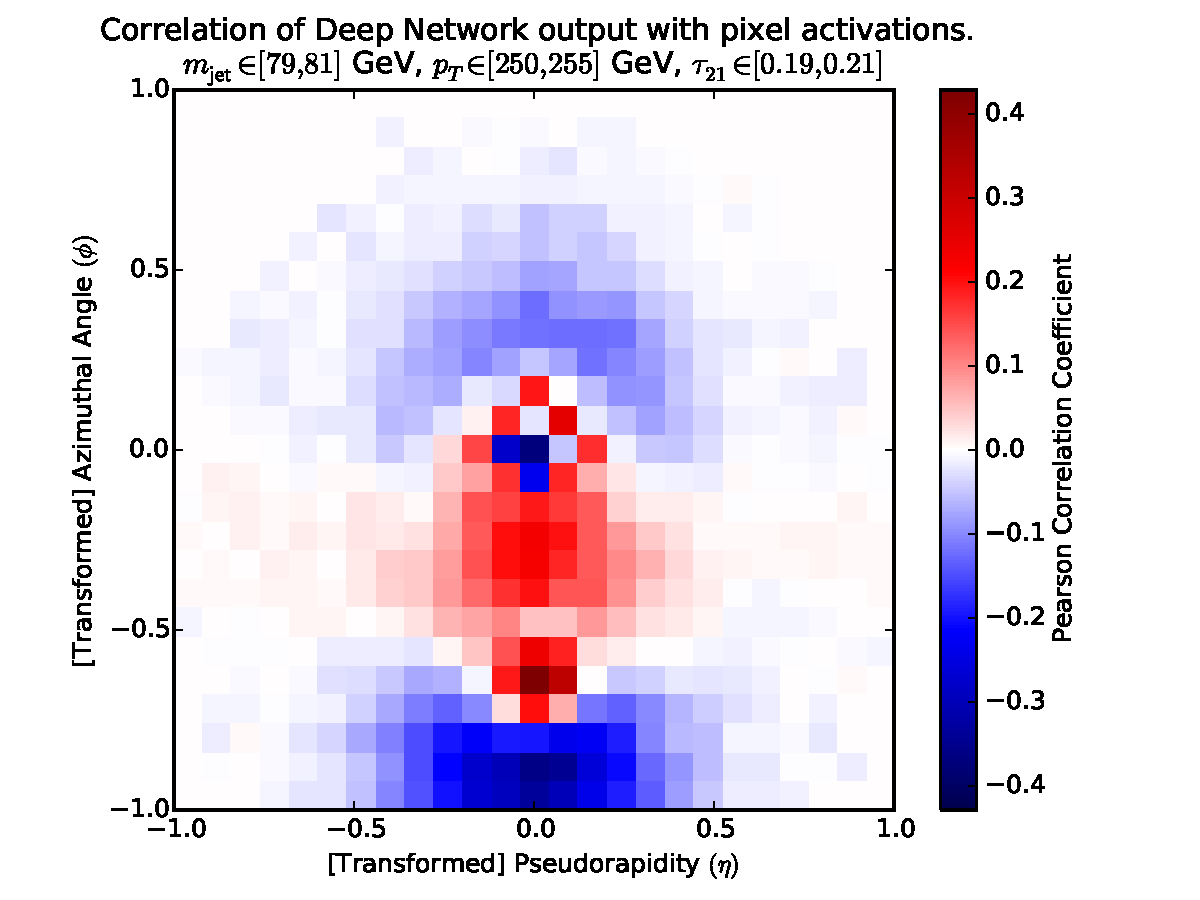
\includegraphics[width=0.65\textwidth]{figures/pixel-activations-corr-benwindow.pdf}
  \caption{caption}
  \label{fig:corrWindow}
\end{figure}


\begin{figure}[htbp]
  \centering
  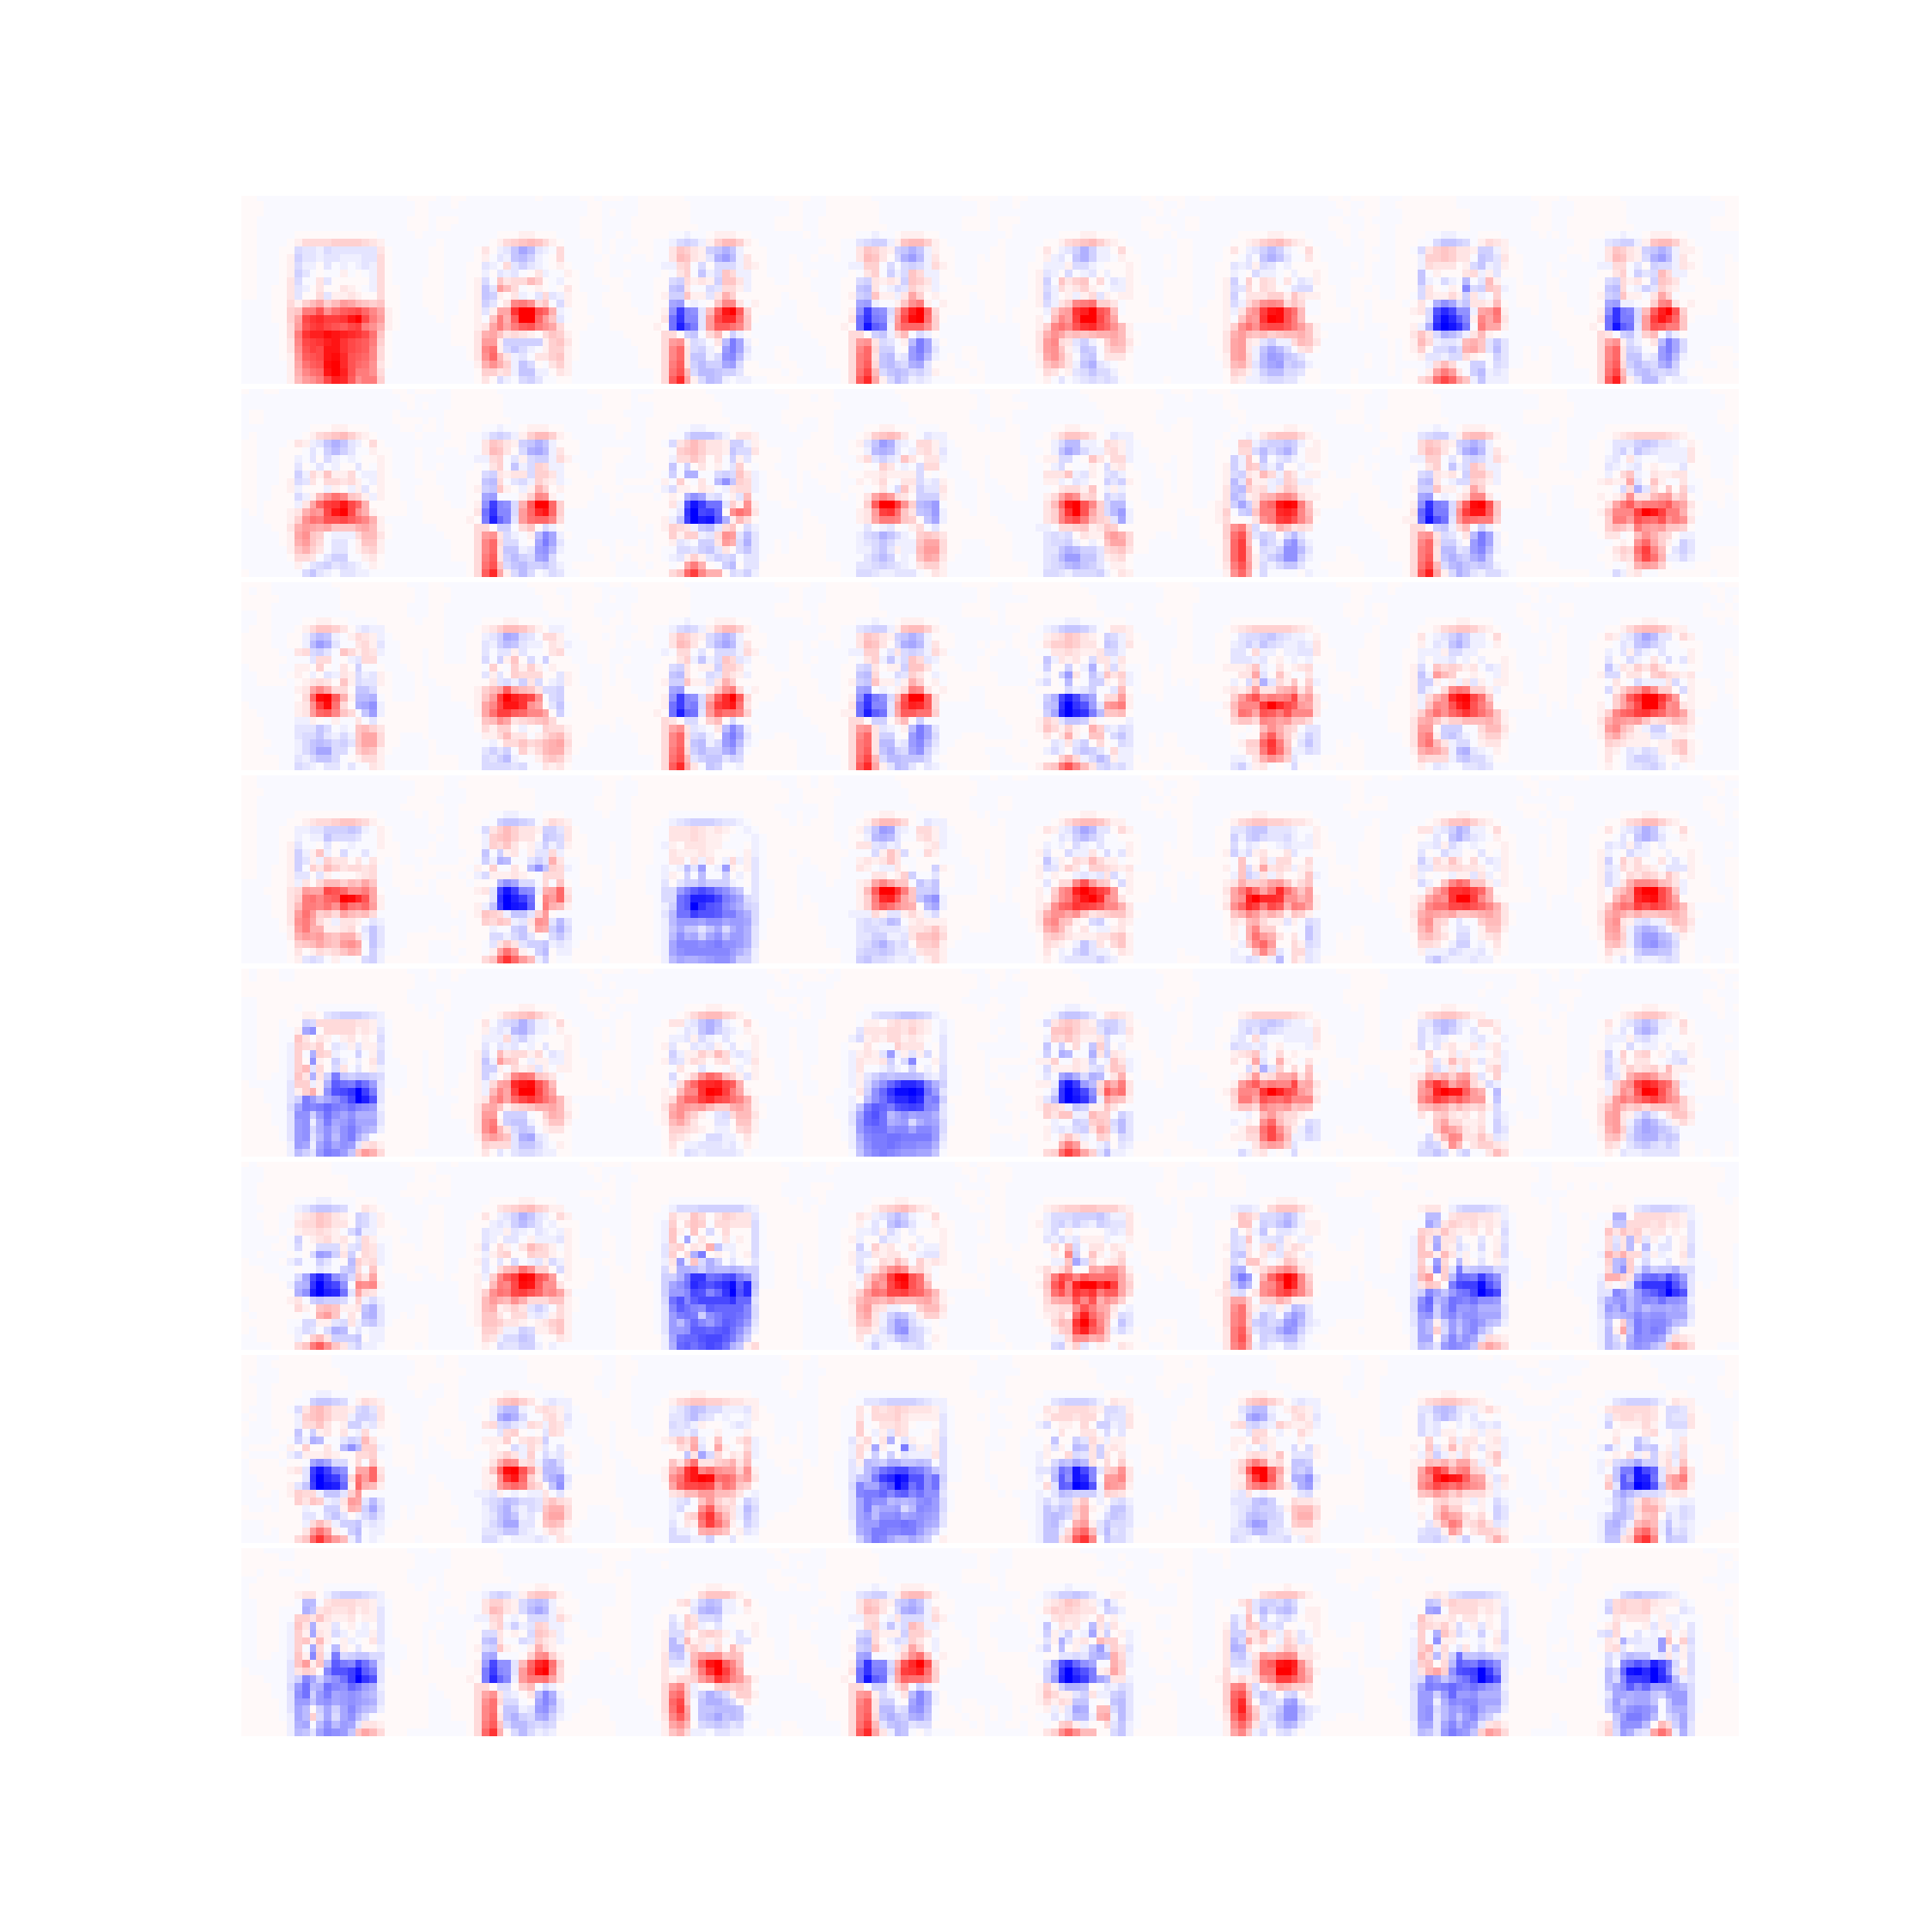
\includegraphics[width=0.95\textwidth]{figures/conv-diffs-ben-window.pdf}
  \caption{caption}
  \label{fig:convkernelsWindow}
\end{figure}
% subsubsection understanding_what_we_learn (end)

% subsection small_window_studies (end)





% section studies (end)


\section{Outlook and Conclusions}
\label{sec:conclusion}
Jet Images are a powerful paradigm for visualizing and classifying jets.  We have shown that when applied directly to jet images, deep neural networks are a powerful tool for identifying boosted hadronically decaying $W$ bosons from QCD multijet processes.  These advanced computer vision algorithms outperform several known and highly discriminating engineered physics-inspired features such as the jet mass and $n$-subjettiness, $\tau_{21}$.  Through a variety of studies, we have shown that some of these features are {\it learned} by the network.  However, despite detailed studies to preserve the jet mass, this important variable seems to not be fully captured by the neural networks studied in this article.  Understanding how to fully learn the jet mass is a goal of our future work.

In this paper, we propose several techniques for quantifying and visualizing the information learned by the DNNs, and connect these visualizations with physics properties.  This is studied by removing the information from jet mass and $\tau_{21}$ through a re-weighting or redaction of the phase space.  In this way, we can evaluate the performance of the network beyond these features to quantify the unique information learned by the network.  In addition to quantifying the amount of additional discrimination achieved by the network, we also show how the new information can be visualized through Fisher jet-images, and through the deep correlation jet image which displays the network output correlation with each input pixel.  These visualizations are a powerful tool for understanding what the network is learning - in this case, colorflow patterns suggest that at least part of the unique information comes from the octet versus singlet nature of $W$ bosons and gluon jets.  These visualizations may even be useful in the future for engineering other simple variables which may be able to match the performance of the neural network.  

This edition of the study of jet images has built a new link between particle physics and computer vision by using state of the art deep neural networks for the classifying high-dimensional high energy physics data.  By processing the raw jet image pixels with these advanced techniques, we have shown that there is a great potential for jet classification.  Many analyses at the LHC use boosted hadronically decaying bosons as probes of physics beyond the Standard Model and the methods presented in this paper have important implications for improving the sensitivity of these analyses.  In addition to improving tagging capabilities, further studies with deep neural networks will help us discover new features to improve our understanding and improve upon existing features to fully capture the wealth of information inside jets.

\section{Acknowledgements} % (fold)
\label{sec:acknowledgements}

We would like to thank Andrew Larkoski for useful conversations about the physics observed in the jet images.  This work is supported by the Stanford Data Science Initiative and by the US Department of Energy (DOE) under grant DE-AC02-76SF00515. BN is supported by the NSF Graduate Research Fellowship under Grant No. DGE-4747 and by the Stanford Graduate Fellowship.  

% section acknowledgements (end)



\clearpage
\newpage

% \nocite{*}
 \bibliography{myrefs}





\end{document}
